\documentclass[conference]{IEEEtran}
\usepackage[x11names, svgnames, rgb]{xcolor}
\usepackage[utf8]{inputenc}
\usepackage{amsmath, amssymb, amsthm,tikz, subfig}
\usetikzlibrary{positioning,shapes,quotes,calc,snakes,arrows}

\newtheorem{theorem}{Theorem}[section]
\newtheorem{corollary}{Corollary}[theorem]
\newtheorem{lemma}{Lemma}[section]
\theoremstyle{definition}
\newtheorem{definition}{Definition}[section]
\newtheorem{example}{Example}[section]
\theoremstyle{remark}
\newtheorem{remark}{Remark}[section]

\usepackage{algorithm, algpseudocode}
\algrenewcommand\algorithmicrequire{\textbf{Input:}}
\algrenewcommand\algorithmicensure{\textbf{Output:}}

\usepackage{scalerel}
\DeclareMathOperator*{\bigplus}{\scalerel*{+}{\sum}}

\usepackage[strings]{underscore} % fixes doi underscores
\usepackage{hyperref} % brings up so many errors
\usepackage[capitalise, noabbrev]{cleveref}
\usepackage{mathrsfs} %for mathscr

\newcommand{\AP}{\mathcal{AP}}
\newcommand{\always}{\Box}
\newcommand{\eventually}{\Diamond}
\newcommand{\nextt}{\mathcal{X}}
\newcommand{\limplies}{\rightarrow}
\newcommand{\ltl}{\textit{LTL}}

\newcommand{\tand}{\land}
\newcommand{\tor}{\lor}
\newcommand{\tnot}{\lnot}

\newcommand{\Buchi}{B\"{u}chi }
\newcommand{\stronguntil}{\hspace{0.1cm} \mathcal{U}  \hspace{0.1cm}}
\newcommand{\strongrelease}{\hspace{0.1cm} \mathcal{M} \hspace{0.1cm}}
\newcommand{\weakuntil}{\hspace{0.1cm} \mathcal{W} \hspace{0.1cm}}
\newcommand{\weakrelease}{\hspace{0.1cm} \mathcal{R} \hspace{0.1cm}}
\newcommand{\liff}{\leftrightarrow}

%\newcommand{\tool}{\hspace{0.1cm}\texttt{ltl2timeline}\hspace{0.1cm}}
\newcommand{\tool}{\texttt{ltl2timeline}}

\newcommand{\tllen}{\text{tllen}}

\renewcommand{\phi}{\varphi}

\renewcommand{\L}{\mathscr{L}}

\tikzset{
    partial ellipse/.style args={#1:#2:#3}{
        insert path={+ (#1:#3) arc (#1:#2:#3)}
    }
}

\begin{document}


\title{What's in a Name? \\ Linear Temporal Logic \\ Literally Represents Time Lines}

\author{\IEEEauthorblockN{Runming Li\textsuperscript{\textsection}}
\IEEEauthorblockA{\textit{Carnegie Mellon University}\\
Pittsburgh, PA, USA \\
runmingl@andrew.cmu.edu}
\and
\IEEEauthorblockN{Keerthana Gurushankar\textsuperscript{\textsection}}
\IEEEauthorblockA{\textit{Carnegie Mellon University}\\
Pittsburgh, PA, USA \\
kgurusha@andrew.cmu.edu}
\and
\IEEEauthorblockN{Marijn~J.H.~Heule}
\IEEEauthorblockA{\textit{Carnegie Mellon University}\\
Pittsburgh, PA, USA \\
marijn@cmu.edu}
\and
\IEEEauthorblockN{Kristin~Yvonne~Rozier}
\IEEEauthorblockA{\textit{Iowa State University} \\
Ames, IA, USA \\
kyrozier@iastate.edu}
}

\maketitle
\begingroup\renewcommand\thefootnote{\textsection}
\footnotetext{These authors contributed equally to this work}
\endgroup

\thispagestyle{plain}
\pagestyle{plain}
\pagenumbering{gobble}


\begin{abstract}
  Linear Temporal Logic (LTL) is arguably the most popular specification language for formal verification of safety-critical systems.
  However, LTL formulas can be unintuitive and error-prone for human practitioners to specify and validate. Meanwhile, drawing timelines remains one of the most popular methods for specifying and validating requirements for industrial system designs, such as in aerospace operational concepts.
  Therefore, we provide a new timeline tool for visualizing LTL specifications as timelines, providing provably-correct, intuitive equivalents between these two specification formats.
  Our tool generates timeline visualizations by translating LTL formulas to intermediate representations as B\"{u}chi automata and then regular expressions, and finally simplifying and visualizing the expressions.
  We provide an algorithm for this visualization, a theoretical soundness analysis, and an implementation.
\end{abstract}

\begin{IEEEkeywords}
Modal and Temporal Logics, Logic and Verification, Regular languages
\end{IEEEkeywords}

%\section{Introduction}
\section{Prologue} %going full Shakespeare on this...
Requirement specification is a central step in the development of safety-critical systems. %As a first step, requirements are typically written in natural language.
For example, here is a real-world requirement specification from an air traffic control system~\cite{ZR14}
\begin{center}
    ``If a TSAFE command is sent to an aircraft, controller/AutoResolver should then hand off the control of this aircraft''
\end{center}
Such natural language requirements are often ambiguous and not amenable to formal analysis, so we must instead specify such requirements using rigorous formalized semantics for the purpose of verification and validation. The above requirement, when translated to Linear Temporal Logic (detailed in \cref{sec:ltl}), may be expressed as follows:
\begin{align*}
    \always & (\texttt{tsafe.TSAFE\_command1} \land \\ & \texttt{controller.CTR\_control\_1} \\
    \limplies & \nextt (\neg \texttt{controller.CTR\_control\_1}))
\end{align*}
Though, as \cite{ZR14} demonstrates, validating that the resulting formula represents the intended requirement is difficult, even for professionals; in this case study a subtle misconception in the initial formalization of a requirement hid an important safety concern present in the early design-stage requirements. Using the play-on-words "Little Tricky Logic," \cite{GSNK22} points to endemic misconceptions in the understanding of LTL.

The need for validation of requirements formalizations has been widely recognized, and tools for several different formalisms have contributed strategies for breaking up the formalisms into patterns and adding GUIs to make validation easier. For example, the web-based modeling tool piStar-ext adds a GUI with text, symbols, and diagrams to enable users to better validate iStar-language models \cite{GRMPAC20}. Hanfor, a GUI, web-based tool supported formalization of system requirements into an LTL-like structured natural language patterns for several industry projects in the automotive and railway domains \cite{BDHHLPW21}.
The ForeMoSt framework enables validation of safety assurance cases by translating structured arguments into formal strategies and validating them automatically using the Lean theorem prover \cite{VMDMSC22}.
AutoTap provides users with a GUI utilizing structured English to write and edit LTL formulas representing Trigger-Action Programs (another form of assume-guarantee contracts) for smart devices and cloud services \cite{ZHMBLU19}.

There has been a recent boom in validation capabilities for the related, but arguably simpler, specification logic Mission-time LTL (MLTL) \cite{LVR19}, which adds finite, integer-bounded, closed intervals to the temporal operators of LTL. The runtime verification engine R2U2 includes a web-based GUI enabling specifiers to visualize properties of (sets of) MLTL runtime monitors, such as their shared subformulas and resource usage on embedded systems \cite{JJKRZ23}. The FRET tool's GUI color-codes segments of structured natural language to elicit more accurate MLTL formulas from system designers \cite{GPMS20}. The WEST tool provides an interactive GUI for MLTL formula validation via regular expressions and truth-table-like visualizations \cite{EGSTWR23}. Now we need tools like these for LTL.

The common and intuitive technique of validating LTL formulas via sets of positive and negative examples (i.e., demonstrating traces that both satisfy and violate a given LTL formula) is insufficient for understanding and explainability of LTL specification \cite{NR22}.
Thus, a significant hurdle remains: how can we convincingly demonstrate to the humans in the loop, from system designers to certifiers, that the analyzed formulas truly represent the desired system requirements? % quote MLTL paper?

We take a simple idiomatic approach to address this problem. Since Linear Temporal Logic formulas differentiate temporal information, we devise a tool, \tool, which can draw timelines to depict the satisfying traces of the LTL formula, and thereby represent the specified behavior in a more natural, human-intelligible form.

Our tool, \tool, uses a remarkably simple algorithm: transforming an input LTL formula through a sequence of automata and regular expression-based intermediate representations. Yet, it is surprisingly effective at providing small representations for a range of LTL formulas. It visualizes the above air traffic control requirement behavior with the timeline shown in \cref{example:air}.

We make the following contributions in our paper:
\begin{itemize}
    \item We provide the tool, \tool, which takes LTL formulas and synthesizes timeline visualizations for them.
    \item We prove correctness in \cref{sec:analysis}. We show that for every LTL formula, the timeline outputted indeed represents the set of satisfying traces.
    \item We showcase the results of our tool on a range of example formulas from real-life industrial verification efforts in \cref{sec:tool-showcase} and \cref{sec:playing}, including discussing the air traffic control example above.
\end{itemize}

\section{Setting the stage}

We begin by setting up the prerequisite definitions involved in our work.
First, we provide the definition and semantics for LTL. In the following subsections, we define (state-based) \Buchi automata and $\omega$-regular expressions, which are generalizations of the well-known deterministic finite automata (DFA) and regular expressions, for the case of infinite words. Lastly, we describe the graphic visualizations we will use to depict timelines.

\subsection{Linear Temporal Logic (LTL)} \label{sec:ltl}

\begin{definition}[Linear Temporal Logic (LTL)]
    % cite Kristin's survey paper
    The syntax of an LTL formula over a set of atomic propositions $\AP$, where $p\in\AP$ is a propositional variable, consists of the following grammar:
    \begin{align*}
        \varphi = & p \mid \neg \varphi \mid \varphi \land \psi \mid \varphi \lor \psi \mid \varphi \limplies \psi \mid \always \varphi \mid \eventually \varphi \mid \nextt \varphi \\ & \mid \varphi \stronguntil \psi \mid \varphi \weakrelease \psi
    \end{align*}\label{ltl-defn}
\end{definition}

\begin{remark}
    Intuitively, $\always \varphi$ says that formula $\varphi$ is true at every time step; $\eventually \varphi$ says that formula $\varphi$ is true either now or at some time in the future; $\nextt \varphi$ says formula $\varphi$ is true at the next time step immediately after the current one; $\varphi \stronguntil \psi$ says that formula $\varphi$ is true \textit{until} (strictly before) such time formula $\psi$ becomes true (and $\psi$ is either true now or in the future); and $\varphi \weakrelease \psi$ says that formula $\psi$ must be true now and remain true unless formula $\varphi$ becomes true, after which point we can \textit{release} $\psi$ (if formula $\phi$ is never true, then formula $\psi$ must remain true at all times).
\end{remark}

\begin{remark}
    The \tool\ tool uses a concrete input syntax of ASCII symbols to represent those logical connectives, in order to simplify typesetting connectives such as $\always$ and $\eventually$. For reference, the concrete syntax appears in Appendix ~\ref{sec:concrete-syntax}.
\end{remark}

\begin{definition}[Semantics of LTL]
    Let $\pi : \omega \rightarrow 2^{\AP}$ be a \emph{computation} or trace that stores the truthhood and falsehood of every atomic proposition at every time step, where $\omega$ is the set of natural numbers that label the time step.
    Then we say $\pi, i \models \varphi$, that is, computation $\pi$ starting from time $i \in \omega$ models LTL formula $\phi$ whenever the result of this evaluation satisfies $\phi$; see Rozier~\cite{Roz11} for the full LTL semantics.
\end{definition}

\subsection{State-based \Buchi automata (BA)}
\begin{definition}[$\omega$-word]
    Let $\Sigma$ be an alphabet. An $\omega$-word or infinite run of $\Sigma$, is an infinite string $s = (s_0, s_1, s_2, \dots)$ where each $s_i\in \Sigma$.
\end{definition}
\begin{definition}[\Buchi automaton (BA)]
    A \Buchi automaton is a $5$-tuple, $(Q, \Sigma, \delta, s, F)$ consisting of
    \begin{enumerate}
        \item a finite set of states $Q$
        \item a finite alphabet of input symbols $\Sigma$
        \item a transition relation $\delta \subseteq (Q\times \Sigma) \times Q$
        \item an initial or start state called $s\in Q$
        \item a set of accepting states $F \subseteq Q$
    \end{enumerate}
    A BA accepts an infinite run iff at least one of its infinitely visited states is in $F$.
\end{definition}

\subsection{$\omega$-regular expressions}
\begin{definition}[Regular expression]\label{def:regex}
    Let $a$ be a symbol in $\Sigma$, $A$ be a regular expression, and $\epsilon$ be the empty expression. We define regular expressions using the following grammar:
    \begin{align*}
        A = \emptyset \mid \epsilon \mid a \mid AA \mid A + A \mid A^*
    \end{align*}
\end{definition}
\begin{definition}[Semantics of regular expressions]
    Let $\L(A)$ denote the set of propositional formulas accepted by regular expression $A$, also called the language accepted by $A$. We define $\L(A)$, inductively as:
    \begin{align*}
        \L(\emptyset) & = \emptyset \\
        \L(\epsilon) & = \{\epsilon\} \tag{$\epsilon$ denotes the empty string}\\
        \L(a) & = \{a\} \\
        \L(A_1A_2) & = \{s_1s_2 \mid s_1 \in L(A_1) \text{ and } s_2 \in L(A_2)\} \\
        \L(A_1 + A_2) & = L(A_1) \cup L(A_2) \\
        \L^{(0)}(A) & = \{\epsilon\} \\
        \L^{(i + 1)}(A) & = \{s_1s_2 \mid s_1 \in L(A) \text{ and } s_2 \in L^{(i)}(A)\} \\\
        \L(A^*) & = \bigcup_{i \ge 0} L^{(i)}(A)
    \end{align*}
\end{definition}

\begin{remark}
    For the purpose of our tool, we define $\Sigma$ as the set of propositional logic formulas:
    \[
    a \in \Sigma = p \mid \top \mid \bot \mid \neg \phi \mid \phi \land \psi \mid \phi \lor \psi \mid \phi \limplies \psi
    \]
\end{remark}

\begin{definition}[$\omega$-regular expressions]\label{def:omega-regex}
    Our definition \ref{def:regex} of regular expressions concerns only finite-length strings. However, since LTL formulas reason about events that happen over an infinite-length timeline, we need to model them using infinite regular expressions (i.e., $\omega$-regular expressions), which we define via the following grammar:
    \begin{align*}
        B = A^{\omega} \mid AB \mid B + B
    \end{align*}
\end{definition}
\begin{definition}[Semantics of $\omega$-regular expressions]\label{def:omega-semantics}
    Let $\Sigma^{\omega}$ denote the set of infinite-length strings over fixed alphabet $\Sigma$. Let $\L_{\omega}(B)$ denote the $\omega$-language accepted by $\omega$-regular expression $B$. Then we define $\L_{\omega}(B)$ inductively as:
    \begin{align*}
        \L_{\omega}(A^{\omega}) & = \{s_1s_2s_3\cdots \mid s_i \in \L(A) \text{ and } i \ge 1\} \tag{$\epsilon
         \not\in \L(A)$} \\
        \L_{\omega}(AB) & = \{s_1s_2 \mid s_1 \in \L(A) \text{ and } s_2 \in \L_{\omega}(B)\} \\
        \L_{\omega}(B_1 + B_2) &= \L_{\omega}(B_1) \cup \L_{\omega}(B_2)
    \end{align*}
\end{definition}

\begin{remark}
  \Cref{def:regex,def:omega-regex} are the standard definitions of regular expressions and $\omega$-regular expressions, respectively.  We include them here for completeness. For the remainder of the paper, we denote arbitrary regular expressions using $A$ and $\omega$-regular expressions by $B$.
\end{remark}

\subsection{Timelines}\label{sec:timeline}
We present timelines as graphic visualizations containing the following features:
\begin{itemize}
    \item Every timeline starts with a node named ``start.''
    \item Every node represents one time step, and each node has a propositional logic formula $\psi$, which specifies the behavior of atomic propositions at that time step. The formula $\psi$ must be true at that time step. If $\psi = 1$, that means all atomic propositions can behave arbitrarily.
    \item An egg-shaped node with a caption ``repeats $0$ - $\infty$'' means to repeat the (one time step) current node for arbitrarily finitely many times.
    \item A node with label ``$\cdots$'' means to repeat the pattern prior to it and after it arbitrarily finitely many times.
    \item The grey box means repeat infinitely. Once we reach the end of a timeline in the grey box, we must reenter the same grey box from any of its (left) starting points.
    \item Timelines can occur in parallel, signifying that any of the parallel timelines could happen.
\end{itemize}

The manifestation of timelines we use here is one of possibly many timeline representations that we devised for the purpose of visualizing LTL formulas. We show how to construct such timelines from LTL formulas in \cref{sec:correctness-timeline}.

\begin{example}
    In \cref{fig:ex2}, one can reason about two parallel timelines: the upper timeline starts with $p$ holding in the first time step, followed by entering the grey box with one step of $\lnot p$ and one step of $p$. Then at the end of the grey box, we reenter the box, with the next time step being $\lnot p$, and so on. The lower timeline starts with one step of $\lnot p$ and one step of $p$ outside the grey box, and then enters the infinite run of $\lnot p$ and $p$ repeating.
    \begin{figure}[!h]
        \centering
        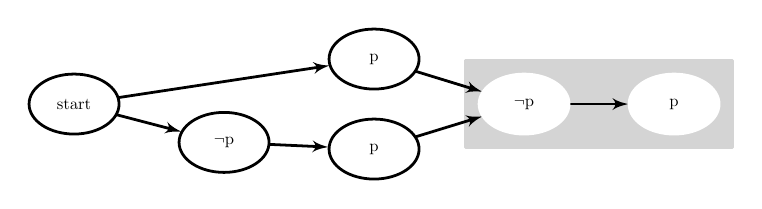
\begin{tikzpicture}[>=latex',line join=bevel,scale=0.6, transform shape]
          \pgfsetlinewidth{1bp}
        %%
        \begin{scope}
          \pgfsetstrokecolor{black}
          \definecolor{strokecol}{rgb}{0.83,0.83,0.83};
          \pgfsetstrokecolor{strokecol}
          \definecolor{fillcol}{rgb}{0.83,0.83,0.83};
          \pgfsetfillcolor{fillcol}
          \filldraw (262.0bp,19.0bp) -- (262.0bp,71.0bp) -- (422.0bp,71.0bp) -- (422.0bp,19.0bp) -- cycle;
        \end{scope}
          \pgfsetcolor{black}
          % Edge: 3 -> 4
          \draw [->] (324.4bp,45.0bp) .. controls (332.06bp,45.0bp) and (340.57bp,45.0bp)  .. (359.62bp,45.0bp);
          % Edge: start -> 0
          \draw [->] (53.503bp,48.868bp) .. controls (83.95bp,53.487bp) and (135.08bp,61.243bp)  .. (180.26bp,68.095bp);
          % Edge: start -> 1
          \draw [->] (52.513bp,38.593bp) .. controls (61.307bp,36.295bp) and (71.403bp,33.656bp)  .. (91.313bp,28.452bp);
          % Edge: 0 -> 3
          \draw [->] (232.05bp,64.622bp) .. controls (241.17bp,61.824bp) and (251.73bp,58.582bp)  .. (271.98bp,52.369bp);
          % Edge: 1 -> 2
          \draw [->] (144.4bp,20.8bp) .. controls (152.06bp,20.452bp) and (160.57bp,20.065bp)  .. (179.62bp,19.199bp);
          % Edge: 2 -> 3
          \draw [->] (232.05bp,25.378bp) .. controls (241.17bp,28.176bp) and (251.73bp,31.418bp)  .. (271.98bp,37.631bp);
          % Node: 3
        \begin{scope}
          \definecolor{strokecol}{rgb}{1.0,1.0,1.0};
          \pgfsetstrokecolor{strokecol}
          \definecolor{fillcol}{rgb}{1.0,1.0,1.0};
          \pgfsetfillcolor{fillcol}
          \filldraw [opacity=1] (297.0bp,45.0bp) ellipse (27.0bp and 18.0bp);
          \definecolor{strokecol}{rgb}{0.0,0.0,0.0};
          \pgfsetstrokecolor{strokecol}
          \draw (297.0bp,45.0bp) node {$\neg \text{p}$};
        \end{scope}
          % Node: 4
        \begin{scope}
          \definecolor{strokecol}{rgb}{1.0,1.0,1.0};
          \pgfsetstrokecolor{strokecol}
          \definecolor{fillcol}{rgb}{1.0,1.0,1.0};
          \pgfsetfillcolor{fillcol}
          \filldraw [opacity=1] (387.0bp,45.0bp) ellipse (27.0bp and 18.0bp);
          \definecolor{strokecol}{rgb}{0.0,0.0,0.0};
          \pgfsetstrokecolor{strokecol}
          \draw (387.0bp,45.0bp) node {$\text{p}$};
        \end{scope}
          % Node: start
        \begin{scope}
          \definecolor{strokecol}{rgb}{0.0,0.0,0.0};
          \pgfsetstrokecolor{strokecol}
          \draw (27.0bp,45.0bp) ellipse (27.0bp and 18.0bp);
          \draw (27.0bp,45.0bp) node {start};
        \end{scope}
          % Node: 0
        \begin{scope}
          \definecolor{strokecol}{rgb}{0.0,0.0,0.0};
          \pgfsetstrokecolor{strokecol}
          \draw (207.0bp,72.0bp) ellipse (27.0bp and 18.0bp);
          \draw (207.0bp,72.0bp) node {$\text{p}$};
        \end{scope}
          % Node: 1
        \begin{scope}
          \definecolor{strokecol}{rgb}{0.0,0.0,0.0};
          \pgfsetstrokecolor{strokecol}
          \draw (117.0bp,22.0bp) ellipse (27.0bp and 18.0bp);
          \draw (117.0bp,22.0bp) node {$\neg \text{p}$};
        \end{scope}
          % Node: 2
        \begin{scope}
          \definecolor{strokecol}{rgb}{0.0,0.0,0.0};
          \pgfsetstrokecolor{strokecol}
          \draw (207.0bp,18.0bp) ellipse (27.0bp and 18.0bp);
          \draw (207.0bp,18.0bp) node {$\text{p}$};
        \end{scope}
        %
        \end{tikzpicture}
   %     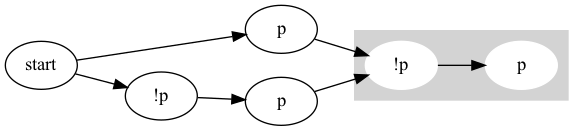
\includegraphics[scale=0.4]{examples/ex2/ex2.png}
        \caption{Example of one possible timeline for the specification ``$p$ oscillates every time step.''}
        \label{fig:ex2}
    \end{figure}
\end{example}

\begin{example}
    In \cref{fig:ex15}, one can reason about one timeline: the atomic proposition $a$ is false for finitely many time steps as signified by the second node (note that this could be zero time steps); followed by one node with $a$ that substantiates the specification of ``$a$ is eventually true.'' Once $a$ is true at some point, the later time steps can behave arbitrarily as signified by the infinite run of $\top$ (true) in the grey box.
    \begin{figure}[!h]
        \centering
        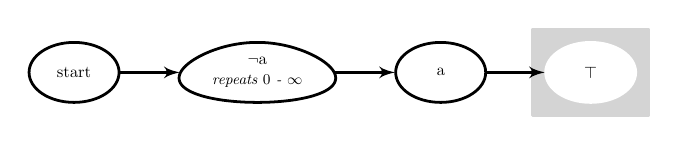
\begin{tikzpicture}[>=latex',line join=bevel,scale=0.6, transform shape]
          \pgfsetlinewidth{1bp}
        %%
        \begin{scope}
          \pgfsetstrokecolor{black}
          \definecolor{strokecol}{rgb}{0.83,0.83,0.83};
          \pgfsetstrokecolor{strokecol}
          \definecolor{fillcol}{rgb}{0.83,0.83,0.83};
          \pgfsetfillcolor{fillcol}
          \filldraw (301.97bp,8.0bp) -- (301.97bp,60.0bp) -- (371.97bp,60.0bp) -- (371.97bp,8.0bp) -- cycle;
        \end{scope}
          \pgfsetcolor{black}
          % Edge: start -> 0
          \draw [->] (54.416bp,34.0bp) .. controls (62.14bp,34.0bp) and (70.893bp,34.0bp)  .. (90.479bp,34.0bp);
          % Edge: 0 -> 1
          \draw [->] (183.47bp,34.0bp) .. controls (191.95bp,34.0bp) and (200.71bp,34.0bp)  .. (219.63bp,34.0bp);
          % Edge: 1 -> 2
          \draw [->] (274.37bp,34.0bp) .. controls (282.03bp,34.0bp) and (290.54bp,34.0bp)  .. (309.58bp,34.0bp);
          % Node: 2
        \begin{scope}
          \definecolor{strokecol}{rgb}{1.0,1.0,1.0};
          \pgfsetstrokecolor{strokecol}
          \definecolor{fillcol}{rgb}{1.0,1.0,1.0};
          \pgfsetfillcolor{fillcol}
          \filldraw [opacity=1] (336.97bp,34.0bp) ellipse (27.0bp and 18.0bp);
          \definecolor{strokecol}{rgb}{0.0,0.0,0.0};
          \pgfsetstrokecolor{strokecol}
          \draw (336.97bp,34.0bp) node {$\top$};
        \end{scope}
          % Node: start
        \begin{scope}
          \definecolor{strokecol}{rgb}{0.0,0.0,0.0};
          \pgfsetstrokecolor{strokecol}
          \draw (27.0bp,34.0bp) ellipse (27.0bp and 18.0bp);
          \draw (27.0bp,34.0bp) node {start};
        \end{scope}
          % Node: 0
        \begin{scope}
          \definecolor{strokecol}{rgb}{0.0,0.0,0.0};
          \pgfsetstrokecolor{strokecol}
          \draw (141.33bp,16.05bp) -- (144.21bp,16.15bp) -- (147.06bp,16.3bp) -- (149.87bp,16.49bp) -- (152.62bp,16.74bp) -- (155.31bp,17.03bp) -- (157.93bp,17.36bp) -- (160.46bp,17.75bp) -- (162.9bp,18.18bp) -- (165.23bp,18.65bp) -- (167.46bp,19.16bp) -- (169.56bp,19.71bp) -- (171.54bp,20.31bp) -- (173.38bp,20.94bp) -- (175.08bp,21.61bp) -- (176.65bp,22.31bp) -- (178.06bp,23.04bp) -- (179.33bp,23.8bp) -- (180.45bp,24.59bp) -- (181.41bp,25.41bp) -- (182.21bp,26.25bp) -- (182.87bp,27.11bp) -- (183.37bp,27.99bp) -- (183.72bp,28.89bp) -- (183.92bp,29.8bp) -- (183.97bp,30.72bp) -- (183.88bp,31.65bp) -- (183.65bp,32.59bp) -- (183.29bp,33.53bp) -- (182.8bp,34.47bp) -- (182.19bp,35.41bp) -- (181.46bp,36.35bp) -- (180.61bp,37.28bp) -- (179.66bp,38.2bp) -- (178.61bp,39.11bp) -- (177.47bp,40.01bp) -- (176.24bp,40.89bp) -- (174.93bp,41.75bp) -- (173.55bp,42.59bp) -- (172.1bp,43.41bp) -- (170.59bp,44.2bp) -- (169.02bp,44.96bp) -- (167.4bp,45.69bp) -- (165.73bp,46.39bp) -- (164.03bp,47.06bp) -- (162.28bp,47.69bp) -- (160.51bp,48.29bp) -- (158.71bp,48.84bp) -- (156.89bp,49.35bp) -- (155.04bp,49.82bp) -- (153.18bp,50.25bp) -- (151.31bp,50.64bp) -- (149.42bp,50.97bp) -- (147.52bp,51.26bp) -- (145.62bp,51.51bp) -- (143.7bp,51.7bp) -- (141.79bp,51.85bp) -- (139.87bp,51.95bp) -- (137.95bp,52.0bp) -- (136.02bp,52.0bp) -- (134.1bp,51.95bp) -- (132.18bp,51.85bp) -- (130.27bp,51.7bp) -- (128.35bp,51.51bp) -- (126.45bp,51.26bp) -- (124.55bp,50.97bp) -- (122.66bp,50.64bp) -- (120.79bp,50.25bp) -- (118.93bp,49.82bp) -- (117.08bp,49.35bp) -- (115.26bp,48.84bp) -- (113.46bp,48.29bp) -- (111.68bp,47.69bp) -- (109.94bp,47.06bp) -- (108.24bp,46.39bp) -- (106.57bp,45.69bp) -- (104.95bp,44.96bp) -- (103.38bp,44.2bp) -- (101.87bp,43.41bp) -- (100.42bp,42.59bp) -- (99.03bp,41.75bp) -- (97.73bp,40.89bp) -- (96.5bp,40.01bp) -- (95.35bp,39.11bp) -- (94.31bp,38.2bp) -- (93.36bp,37.28bp) -- (92.51bp,36.35bp) -- (91.78bp,35.41bp) -- (91.17bp,34.47bp) -- (90.68bp,33.53bp) -- (90.32bp,32.59bp) -- (90.09bp,31.65bp) -- (90.0bp,30.72bp) -- (90.05bp,29.8bp) -- (90.25bp,28.89bp) -- (90.6bp,27.99bp) -- (91.1bp,27.11bp) -- (91.76bp,26.25bp) -- (92.56bp,25.41bp) -- (93.52bp,24.59bp) -- (94.64bp,23.8bp) -- (95.91bp,23.04bp) -- (97.32bp,22.31bp) -- (98.88bp,21.61bp) -- (100.59bp,20.94bp) -- (102.43bp,20.31bp) -- (104.41bp,19.71bp) -- (106.51bp,19.16bp) -- (108.74bp,18.65bp) -- (111.07bp,18.18bp) -- (113.51bp,17.75bp) -- (116.04bp,17.36bp) -- (118.66bp,17.03bp) -- (121.35bp,16.74bp) -- (124.1bp,16.49bp) -- (126.91bp,16.3bp) -- (129.76bp,16.15bp) -- (132.64bp,16.05bp) -- (135.53bp,16.0bp) -- (138.44bp,16.0bp) -- cycle;
          \draw (136.98bp,34.0bp) node [align=center] {$\neg \text{a}$ \\ {\small \emph{repeats $0$ - $\infty$}}};
        \end{scope}
          % Node: 1
        \begin{scope}
          \definecolor{strokecol}{rgb}{0.0,0.0,0.0};
          \pgfsetstrokecolor{strokecol}
          \draw (246.97bp,34.0bp) ellipse (27.0bp and 18.0bp);
          \draw (246.97bp,34.0bp) node {$\text{a}$};
        \end{scope}
        %
        \end{tikzpicture}
    %    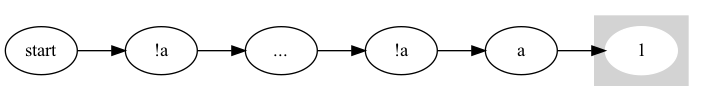
\includegraphics[scale=0.4]{examples/ex15/ex15.png}
        \caption{Example of a timeline for the specification ``$a$ is eventually true.''}
        \label{fig:ex15}
    \end{figure}
\end{example}

\section{Algorithm: ``Though she be but little, she is fierce\textsuperscript{\textsection}''}
\begingroup\renewcommand\thefootnote{\textsection}
\footnotetext{William Shakespeare, \emph{A Midsummer Night's Dream}}
\endgroup
On a high level, our algorithm for converting LTL formulas into timeline visualizations (depicted in \Cref{fig:algo}) works as follows.
\begin{enumerate}
    \item Convert the given LTL formula to its corresponding \Buchi automaton. % (as detailed in \cref{ltl2aut})
    \item Derive the $\omega$-regular expression corresponding to the \Buchi automaton. % (in \cref{aut2regex})
    \item Simplify the derived $\omega$-regular expression. (Note that this step represents a stylistic choice balancing size, complexity, and clarity.) % (in \cref{regex-simplify})
    \item Visualize the $\omega$-regular expression as a timeline according to its structure. %(in \cref{regex2timeline})
\end{enumerate}
\begin{figure*}[!t]
    \centering
    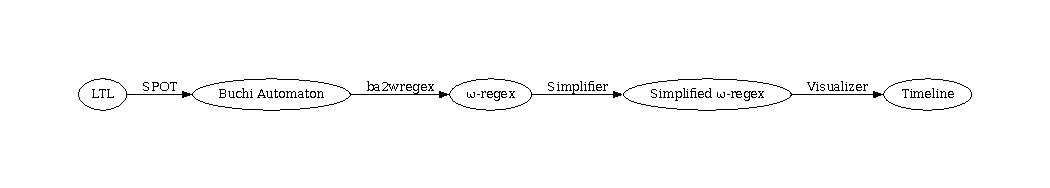
\includegraphics[width=\textwidth, scale=0.3]{img/algorithm_outline.pdf}
    \caption{\tool \ algorithm outline}
    \label{fig:algo}
\end{figure*}

\subsection{LTL to BA} \label{ltl2aut}
The automata-theoretic approach~\cite{ORBi-a8d60ab6-1101-4434-9511-c01ea4e5a15b} to evaluating LTL (e.g., via reducing LTL formulas to their corresponding \Buchi automata) has been well-studied \cite{DGV99,F03,RV10,RV11,Dur14}. Our tool \tool\ uses SPOT~\cite{Dur22}\footnote{We used SPOT version 2.11.} for this step, which provides a provably-correct implementation of the translation from LTL formulas to minimally-sized \Buchi automata.

\subsection{BA to $\omega$-regex} \label{aut2regex}
We translate \Buchi automata to $\omega$-regular expressions by first finding the regular expressions for paths from the start state to some final state (say $r_\mathrm{sf}$), and for those for paths looping from the final state back to itself (say $r_\mathrm{ff}$), and finally combining those to form the $\omega$-expression for satisfying runs $\left(\bigplus_{f\in F} r_\mathrm{sf}r_\mathrm{ff}^\omega\right)$. Our visualization algorithm finds regular expressions for finite paths by iteratively deleting interior nodes in the digraph of the automaton.

%KYR: FIX THIS!
The algorithm is outlined below (see Algorithms 1 - 4). %\cref{alg:ba2wregex}

\begin{algorithm}[h!]
    \caption{reduce\_nfa}
    \begin{algorithmic}
        \Require ($G, v$): NFA $G$ with state $v$ that is not initial or final
        \Ensure Deletes state $v$ from $G$ while ensuring $\L(G)$ remains unchanged
        \For{ every $u\xrightarrow{r_\mathrm{in}} v, v \xrightarrow{r_\mathrm{out}} w$ }
            \If {$v$ has a self-edge  $v\xrightarrow{r_\mathrm{loop}}v$}
                \State replace edges $u\xrightarrow{r_\mathrm{in}} v, v \xrightarrow{r_\mathrm{out}} w$ with $u \xrightarrow{r_\mathrm{in} r_\mathrm{loop}* r_\mathrm{out}} w$
            \Else
                \State replace edges $u\xrightarrow{r_\mathrm{in}} v, v \xrightarrow{r_\mathrm{out}} w$ with $u \xrightarrow{r_\mathrm{in}  r_\mathrm{out}} w$
            \EndIf
        \EndFor
	\State delete node $v$ from $G$
        %\State \Return the reduced graph $G$
    \end{algorithmic}
\end{algorithm}

\begin{algorithm}[h!]
    \caption{nfa2regex}
    \begin{algorithmic}
        \Require ($G, s, f$): NFA $G$ with initial state $s$ and final state $f$
        \Ensure The regular expression corresponding to all paths from $s$ to $f$
        % WHile there exists any edge except r_sf
        \While{ there exists an interior vertex $v$ }
            \State reduce\_nfa($G, v$)
            \State combine multi-edges, i.e., convert $r1 : u \to w, r2 : u \to w$  to $r1 | r2 : u \to w$
        \EndWhile
        \State \Return $(r_\mathrm{ss}| r_\mathrm{sf} r_\mathrm{ff}^* r_\mathrm{fs})^* r_\mathrm{sf} r_\mathrm{ff}$
        % if called by first visit, this is r_\mathrm{ss}* r_\mathrm{sf}
        % if called by ba2wregex, s=f, this is r_\mathrm{ff}
        % consider modularizing fns differently
        % \State \Return regexp labelling the edge $s\to f$
    \end{algorithmic}
\end{algorithm}

\begin{algorithm}[h!]
    \caption{nfa2regex\_firstvisit}
    \begin{algorithmic}
        \Require ($G, s, f$):  NFA $G$ with initial state $s$ and final state $f$
        \Ensure The regular expression of all paths from $s$ reaching $f$ for the first time
        \State delete all out edges from $f$ in $G$
        \State \Return nfa2regex($G, s, f$)
    \end{algorithmic}
\end{algorithm}

\begin{algorithm}[h!]
    \label{alg:ba2wregex}
    \caption{ba2wregex}
    \begin{algorithmic}
        \Require $G$, a \Buchi automaton
        \Ensure The $\omega$-regular expression recognized by $G$
        \State \Return $\bigcup_{f \in F}\left(\text{nfa2regex\_firstvisit}(G, s, f)\text{nfa2regex}(G, f, f) \right) $
    \end{algorithmic}
\end{algorithm}

\subsection{$\omega$-regex simplification} \label{regex-simplify}

The $\omega$-regular expression generated in \cref{aut2regex} may not be the ``simplest'' for the purpose of visualizing the timeline. We have observed multiple patterns in the resulting $\omega$-regular expression that could be simplified. For example, an $\omega$-regular expression of the form of $r^*r^{\omega}$ represents the same timeline as $r^{\omega}$, but the latter is more intuitive and concise. For this purpose, we devised some simplification rules in our tool, based on our observation of common patterns in the generated $\omega$-regular expressions.

There is no agreed-upon canonical form for regular expressions representing LTL formulas, hence we do not hope to find the shortest possible regular expression for visualization. Regular expression simplification comes down to regular expression equivalence checking, which is computationally hard~\cite{MNS04}. For purpose of simplification, one could perform a search over equivalent regular expressions and decide which one is simpler to use. However, this strategy is expensive in terms of the running time, and for the purpose of visualization, we did not use this strategy in our tool. We consider simplification for the purpose of finding the most intuitive regular expression for a given LTL formula to be an interesting direction for future work.

\paragraph*{Rule-based simplification}
Here we show a demonstrating subset of the simplification rules we encoded. In theory one could add more rules to the tool, so long as they are sound; here we only choose to encode the rules that represent common patterns we have observed in the generated $\omega$-regular expressions.
\begin{alignat*}{2}
        & r_1 + r_1r_2^* && \Longrightarrow r_1r_2^* \\
        & r + r && \Longrightarrow r \\
        & r_1 + r_2^*r_1 && \Longrightarrow r_2^*r_1 \\
        & (r^*)^{\omega} && \Longrightarrow r^{\omega} \\
        & (r_1r_2^*)r_2^{\omega} && \Longrightarrow r_1r_2^{\omega} \\
        & (r_1r_2)r_2^{\omega} && \Longrightarrow r_1r_2^{\omega} \\
        & r^*r^{\omega} && \Longrightarrow r^{\omega} \\
        & rr^{\omega} && \Longrightarrow r^{\omega}
\end{alignat*}

\paragraph*{Result of simplification}
These simplification rules lead to more intuitive representations of timelines. Here we demonstrate their effects using an example.

\begin{example}
    Using our algorithm, the LTL formula $\varphi = \always (a \limplies \eventually (\neg a))$ generates the un-simplified $\omega$-regular expression $((\lnot a) | (aa^*(\lnot a)))((\lnot a) | (aa^*(\lnot a)))^{\omega}$, and the simplified version $((\lnot a) | (aa^*(\lnot a)))^{\omega}$, which correspond to the two timelines in \cref{fig:unsimplified} and \cref{fig:simplified}, respectively.
    \begin{figure*}[h!]
        \centering
                \resizebox{\textwidth}{!}{
                    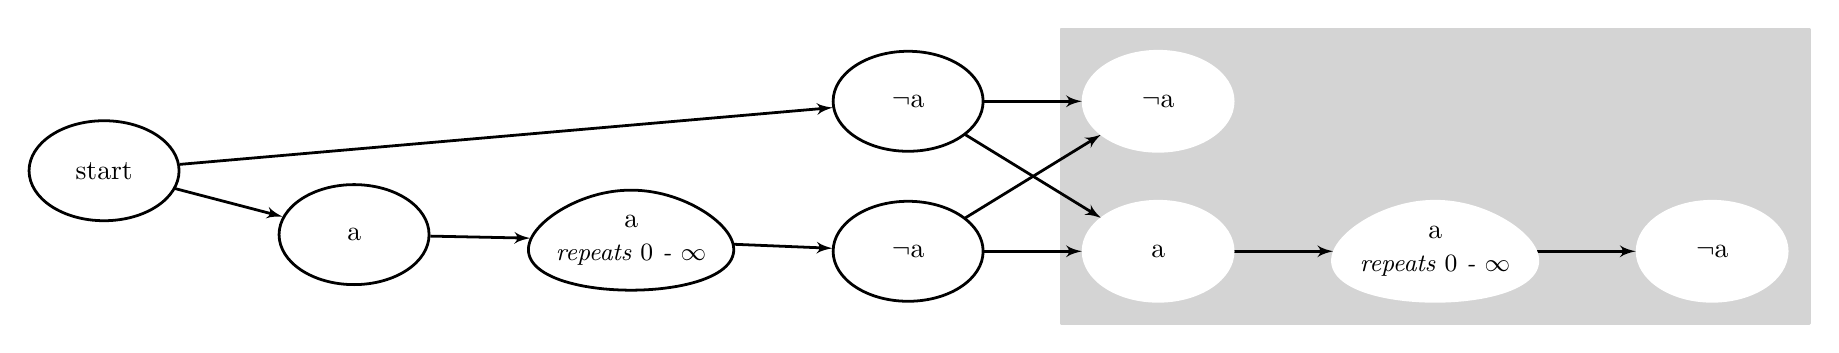
\begin{tikzpicture}[>=latex',line join=bevel,]
                        \pgfsetlinewidth{1bp}
                      %%
                      \begin{scope}
                        \pgfsetstrokecolor{black}
                        \definecolor{strokecol}{rgb}{0.83,0.83,0.83};
                        \pgfsetstrokecolor{strokecol}
                        \definecolor{fillcol}{rgb}{0.83,0.83,0.83};
                        \pgfsetfillcolor{fillcol}
                        \filldraw (371.46bp,8.0bp) -- (371.46bp,114.0bp) -- (640.91bp,114.0bp) -- (640.91bp,8.0bp) -- cycle;
                      \end{scope}
                        \pgfsetcolor{black}
                        % Edge: 5 -> 6
                        \draw [->] (433.9bp,34.0bp) .. controls (441.44bp,34.0bp) and (449.89bp,34.0bp)  .. (469.54bp,34.0bp);
                        % Edge: 6 -> 7
                        \draw [->] (542.74bp,34.0bp) .. controls (550.66bp,34.0bp) and (559.09bp,34.0bp)  .. (578.42bp,34.0bp);
                        % Edge: start -> 0
                        \draw [->] (54.272bp,65.285bp) .. controls (105.49bp,69.739bp) and (218.83bp,79.597bp)  .. (289.35bp,85.729bp);
                        % Edge: start -> 1
                        \draw [->] (52.513bp,56.593bp) .. controls (61.118bp,54.344bp) and (70.969bp,51.769bp)  .. (91.313bp,46.452bp);
                        % Edge: 0 -> 4
                        \draw [->] (343.86bp,88.0bp) .. controls (351.34bp,88.0bp) and (359.64bp,88.0bp)  .. (379.07bp,88.0bp);
                        % Edge: 0 -> 5
                        \draw [->] (336.99bp,76.016bp) .. controls (348.61bp,68.885bp) and (363.57bp,59.705bp)  .. (385.98bp,45.951bp);
                        % Edge: 1 -> 2
                        \draw [->] (144.45bp,39.459bp) .. controls (152.06bp,39.303bp) and (160.61bp,39.128bp)  .. (180.45bp,38.722bp);
                        % Edge: 2 -> 3
                        \draw [->] (253.84bp,36.522bp) .. controls (261.64bp,36.203bp) and (269.9bp,35.864bp)  .. (289.26bp,35.072bp);
                        % Edge: 3 -> 4
                        \draw [->] (336.99bp,45.984bp) .. controls (348.61bp,53.115bp) and (363.57bp,62.295bp)  .. (385.98bp,76.049bp);
                        % Edge: 3 -> 5
                        \draw [->] (343.86bp,34.0bp) .. controls (351.34bp,34.0bp) and (359.64bp,34.0bp)  .. (379.07bp,34.0bp);
                        % Node: 4
                      \begin{scope}
                        \definecolor{strokecol}{rgb}{1.0,1.0,1.0};
                        \pgfsetstrokecolor{strokecol}
                        \definecolor{fillcol}{rgb}{1.0,1.0,1.0};
                        \pgfsetfillcolor{fillcol}
                        \filldraw [opacity=1] (406.46bp,88.0bp) ellipse (27.0bp and 18.0bp);
                        \definecolor{strokecol}{rgb}{0.0,0.0,0.0};
                        \pgfsetstrokecolor{strokecol}
                        \draw (406.46bp,88.0bp) node {$\neg \text{a}$};
                      \end{scope}
                        % Node: 5
                      \begin{scope}
                        \definecolor{strokecol}{rgb}{1.0,1.0,1.0};
                        \pgfsetstrokecolor{strokecol}
                        \definecolor{fillcol}{rgb}{1.0,1.0,1.0};
                        \pgfsetfillcolor{fillcol}
                        \filldraw [opacity=1] (406.46bp,34.0bp) ellipse (27.0bp and 18.0bp);
                        \definecolor{strokecol}{rgb}{0.0,0.0,0.0};
                        \pgfsetstrokecolor{strokecol}
                        \draw (406.46bp,34.0bp) node {$\text{a}$};
                      \end{scope}
                        % Node: 6
                      \begin{scope}
                        \definecolor{strokecol}{rgb}{1.0,1.0,1.0};
                        \pgfsetstrokecolor{strokecol}
                        \definecolor{fillcol}{rgb}{1.0,1.0,1.0};
                        \pgfsetfillcolor{fillcol}
                        \filldraw (509.6bp,16.05bp) -- (511.87bp,16.15bp) -- (514.11bp,16.3bp) -- (516.32bp,16.49bp) -- (518.48bp,16.74bp) -- (520.6bp,17.03bp) -- (522.66bp,17.36bp) -- (524.65bp,17.75bp) -- (526.57bp,18.18bp) -- (528.4bp,18.65bp) -- (530.15bp,19.16bp) -- (531.8bp,19.71bp) -- (533.36bp,20.31bp) -- (534.81bp,20.94bp) -- (536.15bp,21.61bp) -- (537.38bp,22.31bp) -- (538.5bp,23.04bp) -- (539.49bp,23.8bp) -- (540.37bp,24.59bp) -- (541.12bp,25.41bp) -- (541.76bp,26.25bp) -- (542.27bp,27.11bp) -- (542.67bp,27.99bp) -- (542.94bp,28.89bp) -- (543.1bp,29.8bp) -- (543.14bp,30.72bp) -- (543.07bp,31.65bp) -- (542.89bp,32.59bp) -- (542.61bp,33.53bp) -- (542.22bp,34.47bp) -- (541.74bp,35.41bp) -- (541.16bp,36.35bp) -- (540.5bp,37.28bp) -- (539.75bp,38.2bp) -- (538.93bp,39.11bp) -- (538.03bp,40.01bp) -- (537.06bp,40.89bp) -- (536.03bp,41.75bp) -- (534.95bp,42.59bp) -- (533.8bp,43.41bp) -- (532.61bp,44.2bp) -- (531.38bp,44.96bp) -- (530.11bp,45.69bp) -- (528.8bp,46.39bp) -- (527.45bp,47.06bp) -- (526.08bp,47.69bp) -- (524.69bp,48.29bp) -- (523.27bp,48.84bp) -- (521.84bp,49.35bp) -- (520.39bp,49.82bp) -- (518.92bp,50.25bp) -- (517.45bp,50.64bp) -- (515.96bp,50.97bp) -- (514.47bp,51.26bp) -- (512.97bp,51.51bp) -- (511.47bp,51.7bp) -- (509.96bp,51.85bp) -- (508.45bp,51.95bp) -- (506.94bp,52.0bp) -- (505.43bp,52.0bp) -- (503.92bp,51.95bp) -- (502.41bp,51.85bp) -- (500.9bp,51.7bp) -- (499.39bp,51.51bp) -- (497.9bp,51.26bp) -- (496.4bp,50.97bp) -- (494.92bp,50.64bp) -- (493.44bp,50.25bp) -- (491.98bp,49.82bp) -- (490.53bp,49.35bp) -- (489.09bp,48.84bp) -- (487.68bp,48.29bp) -- (486.28bp,47.69bp) -- (484.91bp,47.06bp) -- (483.57bp,46.39bp) -- (482.26bp,45.69bp) -- (480.99bp,44.96bp) -- (479.75bp,44.2bp) -- (478.56bp,43.41bp) -- (477.42bp,42.59bp) -- (476.33bp,41.75bp) -- (475.3bp,40.89bp) -- (474.34bp,40.01bp) -- (473.44bp,39.11bp) -- (472.61bp,38.2bp) -- (471.87bp,37.28bp) -- (471.2bp,36.35bp) -- (470.63bp,35.41bp) -- (470.14bp,34.47bp) -- (469.76bp,33.53bp) -- (469.47bp,32.59bp) -- (469.3bp,31.65bp) -- (469.23bp,30.72bp) -- (469.27bp,29.8bp) -- (469.43bp,28.89bp) -- (469.7bp,27.99bp) -- (470.09bp,27.11bp) -- (470.61bp,26.25bp) -- (471.24bp,25.41bp) -- (472.0bp,24.59bp) -- (472.88bp,23.8bp) -- (473.87bp,23.04bp) -- (474.99bp,22.31bp) -- (476.21bp,21.61bp) -- (477.56bp,20.94bp) -- (479.01bp,20.31bp) -- (480.56bp,19.71bp) -- (482.22bp,19.16bp) -- (483.96bp,18.65bp) -- (485.8bp,18.18bp) -- (487.72bp,17.75bp) -- (489.71bp,17.36bp) -- (491.77bp,17.03bp) -- (493.88bp,16.74bp) -- (496.05bp,16.49bp) -- (498.26bp,16.3bp) -- (500.5bp,16.15bp) -- (502.76bp,16.05bp) -- (505.04bp,16.0bp) -- (507.32bp,16.0bp) -- cycle;
                        \definecolor{strokecol}{rgb}{0.0,0.0,0.0};
                        \pgfsetstrokecolor{strokecol}
                        \draw (506.18bp,34.0bp) node [align=center] {$\text{a}$ \\ {\small \emph{repeats $0$ - $\infty$}}};
                      \end{scope}
                        % Node: 7
                      \begin{scope}
                        \definecolor{strokecol}{rgb}{1.0,1.0,1.0};
                        \pgfsetstrokecolor{strokecol}
                        \definecolor{fillcol}{rgb}{1.0,1.0,1.0};
                        \pgfsetfillcolor{fillcol}
                        \filldraw [opacity=1] (605.91bp,34.0bp) ellipse (27.0bp and 18.0bp);
                        \definecolor{strokecol}{rgb}{0.0,0.0,0.0};
                        \pgfsetstrokecolor{strokecol}
                        \draw (605.91bp,34.0bp) node {$\neg \text{a}$};
                      \end{scope}
                        % Node: start
                      \begin{scope}
                        \definecolor{strokecol}{rgb}{0.0,0.0,0.0};
                        \pgfsetstrokecolor{strokecol}
                        \draw (27.0bp,63.0bp) ellipse (27.0bp and 18.0bp);
                        \draw (27.0bp,63.0bp) node {start};
                      \end{scope}
                        % Node: 0
                      \begin{scope}
                        \definecolor{strokecol}{rgb}{0.0,0.0,0.0};
                        \pgfsetstrokecolor{strokecol}
                        \draw (316.46bp,88.0bp) ellipse (27.0bp and 18.0bp);
                        \draw (316.46bp,88.0bp) node {$\neg \text{a}$};
                      \end{scope}
                        % Node: 1
                      \begin{scope}
                        \definecolor{strokecol}{rgb}{0.0,0.0,0.0};
                        \pgfsetstrokecolor{strokecol}
                        \draw (117.0bp,40.0bp) ellipse (27.0bp and 18.0bp);
                        \draw (117.0bp,40.0bp) node {$\text{a}$};
                      \end{scope}
                        % Node: 2
                      \begin{scope}
                        \definecolor{strokecol}{rgb}{0.0,0.0,0.0};
                        \pgfsetstrokecolor{strokecol}
                        \draw (220.15bp,20.05bp) -- (222.41bp,20.15bp) -- (224.65bp,20.3bp) -- (226.86bp,20.49bp) -- (229.03bp,20.74bp) -- (231.14bp,21.03bp) -- (233.2bp,21.36bp) -- (235.19bp,21.75bp) -- (237.11bp,22.18bp) -- (238.95bp,22.65bp) -- (240.7bp,23.16bp) -- (242.35bp,23.71bp) -- (243.9bp,24.31bp) -- (245.35bp,24.94bp) -- (246.7bp,25.61bp) -- (247.93bp,26.31bp) -- (249.04bp,27.04bp) -- (250.04bp,27.8bp) -- (250.91bp,28.59bp) -- (251.67bp,29.41bp) -- (252.3bp,30.25bp) -- (252.82bp,31.11bp) -- (253.21bp,31.99bp) -- (253.49bp,32.89bp) -- (253.64bp,33.8bp) -- (253.68bp,34.72bp) -- (253.61bp,35.65bp) -- (253.44bp,36.59bp) -- (253.15bp,37.53bp) -- (252.77bp,38.47bp) -- (252.28bp,39.41bp) -- (251.71bp,40.35bp) -- (251.04bp,41.28bp) -- (250.3bp,42.2bp) -- (249.47bp,43.11bp) -- (248.57bp,44.01bp) -- (247.61bp,44.89bp) -- (246.58bp,45.75bp) -- (245.49bp,46.59bp) -- (244.35bp,47.41bp) -- (243.16bp,48.2bp) -- (241.92bp,48.96bp) -- (240.65bp,49.69bp) -- (239.34bp,50.39bp) -- (238.0bp,51.06bp) -- (236.63bp,51.69bp) -- (235.23bp,52.29bp) -- (233.82bp,52.84bp) -- (232.38bp,53.35bp) -- (230.93bp,53.82bp) -- (229.47bp,54.25bp) -- (227.99bp,54.64bp) -- (226.51bp,54.97bp) -- (225.02bp,55.26bp) -- (223.52bp,55.51bp) -- (222.01bp,55.7bp) -- (220.51bp,55.85bp) -- (219.0bp,55.95bp) -- (217.48bp,56.0bp) -- (215.97bp,56.0bp) -- (214.46bp,55.95bp) -- (212.95bp,55.85bp) -- (211.44bp,55.7bp) -- (209.94bp,55.51bp) -- (208.44bp,55.26bp) -- (206.95bp,54.97bp) -- (205.46bp,54.64bp) -- (203.99bp,54.25bp) -- (202.52bp,53.82bp) -- (201.07bp,53.35bp) -- (199.64bp,52.84bp) -- (198.22bp,52.29bp) -- (196.83bp,51.69bp) -- (195.46bp,51.06bp) -- (194.12bp,50.39bp) -- (192.81bp,49.69bp) -- (191.53bp,48.96bp) -- (190.3bp,48.2bp) -- (189.11bp,47.41bp) -- (187.97bp,46.59bp) -- (186.88bp,45.75bp) -- (185.85bp,44.89bp) -- (184.88bp,44.01bp) -- (183.98bp,43.11bp) -- (183.16bp,42.2bp) -- (182.41bp,41.28bp) -- (181.75bp,40.35bp) -- (181.17bp,39.41bp) -- (180.69bp,38.47bp) -- (180.3bp,37.53bp) -- (180.02bp,36.59bp) -- (179.84bp,35.65bp) -- (179.77bp,34.72bp) -- (179.81bp,33.8bp) -- (179.97bp,32.89bp) -- (180.24bp,31.99bp) -- (180.64bp,31.11bp) -- (181.15bp,30.25bp) -- (181.79bp,29.41bp) -- (182.54bp,28.59bp) -- (183.42bp,27.8bp) -- (184.42bp,27.04bp) -- (185.53bp,26.31bp) -- (186.76bp,25.61bp) -- (188.1bp,24.94bp) -- (189.55bp,24.31bp) -- (191.11bp,23.71bp) -- (192.76bp,23.16bp) -- (194.51bp,22.65bp) -- (196.34bp,22.18bp) -- (198.26bp,21.75bp) -- (200.25bp,21.36bp) -- (202.31bp,21.03bp) -- (204.43bp,20.74bp) -- (206.59bp,20.49bp) -- (208.8bp,20.3bp) -- (211.04bp,20.15bp) -- (213.31bp,20.05bp) -- (215.59bp,20.0bp) -- (217.87bp,20.0bp) -- cycle;
                        \draw (216.73bp,38.0bp) node [align=center] {$\text{a}$ \\ {\small \emph{repeats $0$ - $\infty$}}};
                      \end{scope}
                        % Node: 3
                      \begin{scope}
                        \definecolor{strokecol}{rgb}{0.0,0.0,0.0};
                        \pgfsetstrokecolor{strokecol}
                        \draw (316.46bp,34.0bp) ellipse (27.0bp and 18.0bp);
                        \draw (316.46bp,34.0bp) node {$\neg \text{a}$};
                      \end{scope}
                      %
                      \end{tikzpicture}}
%        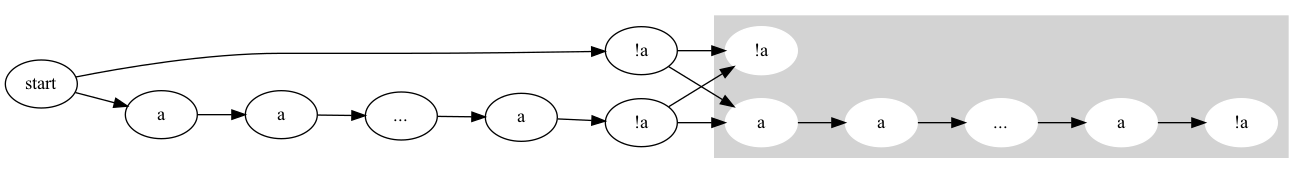
\includegraphics[scale=0.3]{examples/ex9/ex9-unsimplified.png}
        \caption{Timeline visualization for %un-simplified
        $\omega$-regular expression $((\lnot a) | (aa^*(\lnot a)))((\lnot a) | (aa^*(\lnot a)))^{\omega}$.}
        \label{fig:unsimplified}
    \end{figure*}
    \begin{figure*}[h!]
        \centering
        \resizebox{.55\textwidth}{!}{
            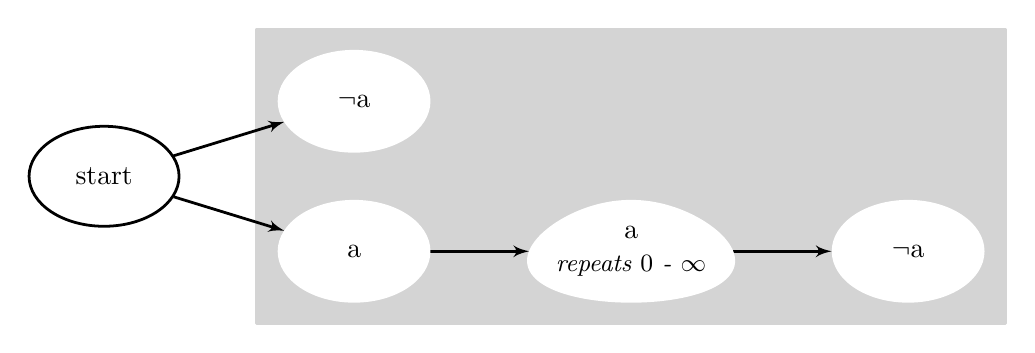
\begin{tikzpicture}[>=latex',line join=bevel,]
                \pgfsetlinewidth{1bp}
              %%
              \begin{scope}
                \pgfsetstrokecolor{black}
                \definecolor{strokecol}{rgb}{0.83,0.83,0.83};
                \pgfsetstrokecolor{strokecol}
                \definecolor{fillcol}{rgb}{0.83,0.83,0.83};
                \pgfsetfillcolor{fillcol}
                \filldraw (82.0bp,8.0bp) -- (82.0bp,114.0bp) -- (351.46bp,114.0bp) -- (351.46bp,8.0bp) -- cycle;
              \end{scope}
                \pgfsetcolor{black}
                % Edge: 1 -> 2
                \draw [->] (144.45bp,34.0bp) .. controls (151.99bp,34.0bp) and (160.43bp,34.0bp)  .. (180.08bp,34.0bp);
                % Edge: 2 -> 3
                \draw [->] (253.29bp,34.0bp) .. controls (261.21bp,34.0bp) and (269.63bp,34.0bp)  .. (288.96bp,34.0bp);
                % Edge: start -> 0
                \draw [->] (52.046bp,68.378bp) .. controls (60.971bp,71.116bp) and (71.285bp,74.281bp)  .. (91.983bp,80.631bp);
                % Edge: start -> 1
                \draw [->] (52.046bp,53.622bp) .. controls (60.971bp,50.884bp) and (71.285bp,47.719bp)  .. (91.983bp,41.369bp);
                % Node: 0
              \begin{scope}
                \definecolor{strokecol}{rgb}{1.0,1.0,1.0};
                \pgfsetstrokecolor{strokecol}
                \definecolor{fillcol}{rgb}{1.0,1.0,1.0};
                \pgfsetfillcolor{fillcol}
                \filldraw [opacity=1] (117.0bp,88.0bp) ellipse (27.0bp and 18.0bp);
                \definecolor{strokecol}{rgb}{0.0,0.0,0.0};
                \pgfsetstrokecolor{strokecol}
                \draw (117.0bp,88.0bp) node {$\neg \text{a}$};
              \end{scope}
                % Node: 1
              \begin{scope}
                \definecolor{strokecol}{rgb}{1.0,1.0,1.0};
                \pgfsetstrokecolor{strokecol}
                \definecolor{fillcol}{rgb}{1.0,1.0,1.0};
                \pgfsetfillcolor{fillcol}
                \filldraw [opacity=1] (117.0bp,34.0bp) ellipse (27.0bp and 18.0bp);
                \definecolor{strokecol}{rgb}{0.0,0.0,0.0};
                \pgfsetstrokecolor{strokecol}
                \draw (117.0bp,34.0bp) node {$\text{a}$};
              \end{scope}
                % Node: 2
              \begin{scope}
                \definecolor{strokecol}{rgb}{1.0,1.0,1.0};
                \pgfsetstrokecolor{strokecol}
                \definecolor{fillcol}{rgb}{1.0,1.0,1.0};
                \pgfsetfillcolor{fillcol}
                \filldraw (220.15bp,16.05bp) -- (222.41bp,16.15bp) -- (224.65bp,16.3bp) -- (226.86bp,16.49bp) -- (229.03bp,16.74bp) -- (231.14bp,17.03bp) -- (233.2bp,17.36bp) -- (235.19bp,17.75bp) -- (237.11bp,18.18bp) -- (238.95bp,18.65bp) -- (240.7bp,19.16bp) -- (242.35bp,19.71bp) -- (243.9bp,20.31bp) -- (245.35bp,20.94bp) -- (246.7bp,21.61bp) -- (247.93bp,22.31bp) -- (249.04bp,23.04bp) -- (250.04bp,23.8bp) -- (250.91bp,24.59bp) -- (251.67bp,25.41bp) -- (252.3bp,26.25bp) -- (252.82bp,27.11bp) -- (253.21bp,27.99bp) -- (253.49bp,28.89bp) -- (253.64bp,29.8bp) -- (253.68bp,30.72bp) -- (253.61bp,31.65bp) -- (253.44bp,32.59bp) -- (253.15bp,33.53bp) -- (252.77bp,34.47bp) -- (252.28bp,35.41bp) -- (251.71bp,36.35bp) -- (251.04bp,37.28bp) -- (250.3bp,38.2bp) -- (249.47bp,39.11bp) -- (248.57bp,40.01bp) -- (247.61bp,40.89bp) -- (246.58bp,41.75bp) -- (245.49bp,42.59bp) -- (244.35bp,43.41bp) -- (243.16bp,44.2bp) -- (241.92bp,44.96bp) -- (240.65bp,45.69bp) -- (239.34bp,46.39bp) -- (238.0bp,47.06bp) -- (236.63bp,47.69bp) -- (235.23bp,48.29bp) -- (233.82bp,48.84bp) -- (232.38bp,49.35bp) -- (230.93bp,49.82bp) -- (229.47bp,50.25bp) -- (227.99bp,50.64bp) -- (226.51bp,50.97bp) -- (225.02bp,51.26bp) -- (223.52bp,51.51bp) -- (222.01bp,51.7bp) -- (220.51bp,51.85bp) -- (219.0bp,51.95bp) -- (217.48bp,52.0bp) -- (215.97bp,52.0bp) -- (214.46bp,51.95bp) -- (212.95bp,51.85bp) -- (211.44bp,51.7bp) -- (209.94bp,51.51bp) -- (208.44bp,51.26bp) -- (206.95bp,50.97bp) -- (205.46bp,50.64bp) -- (203.99bp,50.25bp) -- (202.52bp,49.82bp) -- (201.07bp,49.35bp) -- (199.64bp,48.84bp) -- (198.22bp,48.29bp) -- (196.83bp,47.69bp) -- (195.46bp,47.06bp) -- (194.12bp,46.39bp) -- (192.81bp,45.69bp) -- (191.53bp,44.96bp) -- (190.3bp,44.2bp) -- (189.11bp,43.41bp) -- (187.97bp,42.59bp) -- (186.88bp,41.75bp) -- (185.85bp,40.89bp) -- (184.88bp,40.01bp) -- (183.98bp,39.11bp) -- (183.16bp,38.2bp) -- (182.41bp,37.28bp) -- (181.75bp,36.35bp) -- (181.17bp,35.41bp) -- (180.69bp,34.47bp) -- (180.3bp,33.53bp) -- (180.02bp,32.59bp) -- (179.84bp,31.65bp) -- (179.77bp,30.72bp) -- (179.81bp,29.8bp) -- (179.97bp,28.89bp) -- (180.24bp,27.99bp) -- (180.64bp,27.11bp) -- (181.15bp,26.25bp) -- (181.79bp,25.41bp) -- (182.54bp,24.59bp) -- (183.42bp,23.8bp) -- (184.42bp,23.04bp) -- (185.53bp,22.31bp) -- (186.76bp,21.61bp) -- (188.1bp,20.94bp) -- (189.55bp,20.31bp) -- (191.11bp,19.71bp) -- (192.76bp,19.16bp) -- (194.51bp,18.65bp) -- (196.34bp,18.18bp) -- (198.26bp,17.75bp) -- (200.25bp,17.36bp) -- (202.31bp,17.03bp) -- (204.43bp,16.74bp) -- (206.59bp,16.49bp) -- (208.8bp,16.3bp) -- (211.04bp,16.15bp) -- (213.31bp,16.05bp) -- (215.59bp,16.0bp) -- (217.87bp,16.0bp) -- cycle;
                \definecolor{strokecol}{rgb}{0.0,0.0,0.0};
                \pgfsetstrokecolor{strokecol}
                \draw (216.73bp,34.0bp) node [align=center] {$\text{a}$ \\ {\small \emph{repeats $0$ - $\infty$}}};
              \end{scope}
                % Node: 3
              \begin{scope}
                \definecolor{strokecol}{rgb}{1.0,1.0,1.0};
                \pgfsetstrokecolor{strokecol}
                \definecolor{fillcol}{rgb}{1.0,1.0,1.0};
                \pgfsetfillcolor{fillcol}
                \filldraw [opacity=1] (316.46bp,34.0bp) ellipse (27.0bp and 18.0bp);
                \definecolor{strokecol}{rgb}{0.0,0.0,0.0};
                \pgfsetstrokecolor{strokecol}
                \draw (316.46bp,34.0bp) node {$\neg \text{a}$};
              \end{scope}
                % Node: start
              \begin{scope}
                \definecolor{strokecol}{rgb}{0.0,0.0,0.0};
                \pgfsetstrokecolor{strokecol}
                \draw (27.0bp,61.0bp) ellipse (27.0bp and 18.0bp);
                \draw (27.0bp,61.0bp) node {start};
              \end{scope}
              %
              \end{tikzpicture}}
  %      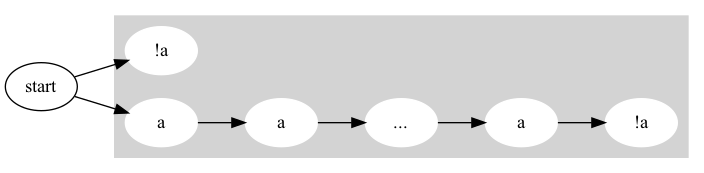
\includegraphics[scale=0.3]{examples/ex9/ex9.png}
        \caption{Timeline visualization for simplified $\omega$-regular expression $((\lnot a) | (aa^*(\lnot a)))^{\omega}$.}
        \label{fig:simplified}
    \end{figure*}
\end{example}

\begin{remark}
    Both simplified and un-simplified $\omega$-regular expressions could generate correct timeline representations that faithfully represent the set of satisfying traces of the original LTL formula $\varphi$. Nonetheless, we, as human users, oftentimes find the simplified version more intuitive to reason about.
\end{remark}

\subsection{$\omega$-regex to timeline} \label{regex2timeline}
Our tool uses Graphviz~\cite{Ellson2001GraphvizO} to achieve the timeline visualization step. By construction of our algorithm, every $\omega$-regular expression is in the form of
\[
    A_1A_2^{\omega} + A_3A_4^{\omega} + \cdots + A_{2n-1}A_{2n}^{\omega}
\]
where $A_i$ are regular expressions, $A_{2i-1}$ could be $\epsilon$, and $\epsilon \not\in \L(A_{2i})$. At a high level, we visualize each regular expression $A_i$ as a set of accepted inputs. We view each union operator as a set of parallel timelines. We denote that each $A_{2i-1}$ gets concatenated with $A_{2i}$, which then repeats infinitely many times by surrounding these repeating final nodes with grey boxes. \cref{fig:timeline} presents a generic timeline resulting from this construction pattern.
\begin{figure}[h!]
    \centering
    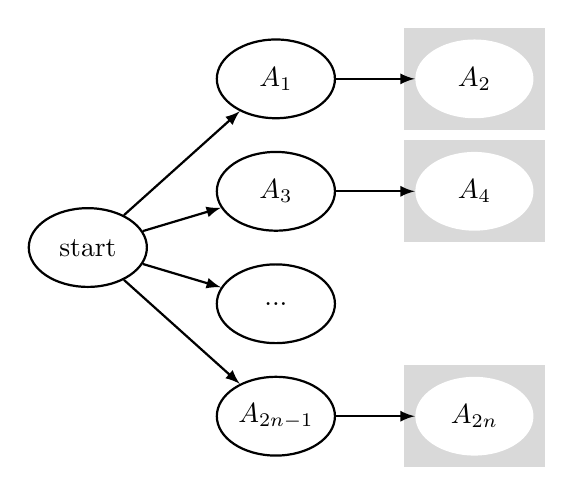
\begin{tikzpicture}
    \node[draw, thick, fill=white, shape=ellipse, style={minimum width=1.5cm, minimum height=1cm}] (a1) {$A_1$};
    \node[shape=rectangle, fill=gray!30!white, style={minimum width=1.8cm, minimum height=1.3cm}] (a2g) [right= 0.85cm of a1] {};
    \node[fill=white, shape=ellipse, style={minimum width=1.5cm, minimum height=1cm}] (a2) [right= 1cm of a1] {$A_2$};
    \node[draw, thick, shape=ellipse, style={minimum width=1.5cm, minimum height=1cm}] (a3) [below= 0.4cm of a1] {$A_3$};
    \node[shape=rectangle, fill=gray!30!white, style={minimum width=1.8cm, minimum height=1.3cm}] (a4g) [right= 0.85cm of a3] {};
    \node[fill=white, shape=ellipse, style={minimum width=1.5cm, minimum height=1cm}] (a4) [right= 1cm of a3] {$A_4$};
    \node[draw, thick, fill=white, shape=ellipse, style={minimum width=1.5cm, minimum height=1cm}] (a5) [below= 0.4cm of a3] {...};
    \node[draw, thick, fill=white, shape=ellipse, style={minimum width=1.5cm, minimum height=1cm}] (a7) [below= 0.4cm of a5] {\!\!\!$A_{2n-1}$\!\!\!};
    \node[shape=rectangle, fill=gray!30!white, style={minimum width=1.8cm, minimum height=1.3cm}] (a8g) [right= 0.85cm of a7] {};
    \node[fill=white, shape=ellipse, style={minimum width=1.5cm, minimum height=1cm}] (a8) [right= 1cm of a7] {\!\!\!$A_{2n}$\!\!\!};
    \node (m) at ($(a1)!0.5!(a7)$) {};
    \node[draw, thick, fill=white, shape=ellipse, style={minimum width=1.5cm, minimum height=1cm}] (s) [left= 1.5cm of m] {\!\!\!\!start\!\!\!\!};
    \draw[thick] (s) edge[-latex] (a1) (s) edge[-latex] (a3) (s) edge[-latex] (a5) (s) edge[-latex] (a7);
    \draw[thick] (a1) edge[-latex] (a2) (a3) edge[-latex] (a4) (a7) edge[-latex] (a8);
    \end{tikzpicture}
%    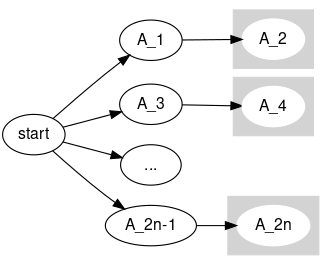
\includegraphics[scale=0.5]{img/timeline.png}
    \caption{Generic timeline construction created from $A_1A_2^{\omega} + A_3A_4^{\omega} + \cdots + A_{2n-1}A_{2n}^{\omega}$.}
    \label{fig:timeline}
\end{figure}

%\section{Theoretical Analyses} \label{sec:analysis}
\section{Theoretical Analyses: ``If we are true to ourselves, we can not be false to anyone\textsuperscript{\textsection}''}
\label{sec:analysis}
\begingroup\renewcommand\thefootnote{\textsection}
\footnotetext{William Shakespeare, \emph{Hamlet}}
\endgroup

We prove the correctness of our translation pipeline. The correctness of the translation from LTL formulas to \Buchi automata stems from using SPOT~\cite{Dur22}. Below, we prove the correctness of (i) the translation from \Buchi automata to $\omega$-regular expressions, and (ii) the ($\omega$-)regular expression rewrite rules we apply. Lastly, we outline the correctness of our timeline visualizations.
\subsection{Correctness of Regex Translation}
\begin{lemma}
    % reduce_nfa does its input to output behaviour
    For any NFA $G$ and any state $v$ in $G$ that is neither a start state or a final state, \textbf{reduce\_nfa}$(G, v)$ preserves the regular language accepted by $G$.
\end{lemma}
\begin{proof}
    Let $G'$ be the graph of $G$ post reduction by the application of \textbf{reduce\_nfa}$(G, v)$. We show that the trace of every path accepted by $G$ is also accepted by $G'$. Suppose a path accepted by $G$ does not pass through $v$, clearly the lemma holds. Otherwise, suppose the path passes through $v$; since $v$ is an interior node, $v$ cannot be the first or last in the path. Thus, for every pass through $v$, let $u\neq v$ be the last node passed before entering $v$, and likewise $w$ be the first node after exiting $v$. We show that the regular language of sub-traces from $u$ to $w$ in $G$ (shown in \cref{fig:uvw-dfa}) is identical to that in $G'$.
    \begin{figure}[h!]
        \centering
        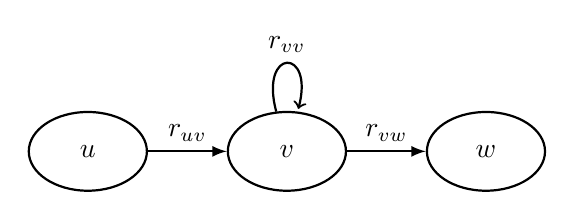
\begin{tikzpicture}
	\node[draw, thick, shape=ellipse, style={minimum width=1.5cm, minimum height=1cm}] (u) {$u$};
	\node[draw, thick, shape=ellipse, style={minimum width=1.5cm, minimum height=1cm}] (v) [right=of u] {$v$};
	\node[draw, thick, shape=ellipse, style={minimum width=1.5cm, minimum height=1cm}] (w) [right=of v] {$w$};
	\draw[thick] (u) edge["$r_{uv}$",-latex] (v) (v) edge["$r_{vv}$",-latex,loop above] (v) (v) edge["$r_{vw}$",-latex] (w);
        \end{tikzpicture}
 %       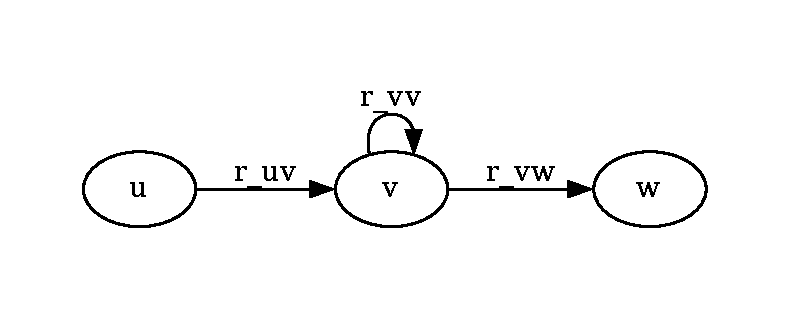
\includegraphics[scale=0.75]{img/uvw_dfa.pdf}
        \caption{A path from $u$ to $w$ in $G$.}
        \label{fig:uvw-dfa}
    \end{figure}
    Suppose there is no loop at $v$, the path from $u$ to $w$ must simply be $u\xrightarrow{r_{uv}}v\xrightarrow{r_{vw}}w$, with the trace $r=r_{uv}r_{vw}$. If there is a loop edge $r_{vv}$, this edge can be traveled any number of times before exiting $v$, thus the regular expression is $r=r_{uv}r_{vv}^*r_{vw}$. This edge $u\xrightarrow{r}w$ was added to $G'$. Thus, for every path accepted by $G$, for every subpath entering and exiting $v$ from some $u$ to $w$, there exists a corresponding subpath from $u$ to $w$ in $G'$, and thus a corresponding path accepted by $G'$.
\end{proof}

\begin{lemma}
    For any NFA $G$ with start state $s$ and (exactly one) final state $f$, \textbf{nfa2regex}$(G, s, f)$ outputs the regular expression capturing all paths from $s$ to $f$ (i.e., $\L(G)$, the language accepted by $G$).
\end{lemma}
\begin{proof}
    The {\bf while} loop clearly terminates since the number of interior nodes is strictly decreasing, and upon termination, $G$ is an NFA containing only the nodes $s$ and $f$. Now, every non-terminal visit from $s$ to $f$ and back to $s$, can be replaced by an edge $s\xrightarrow{r_\mathrm{sf}r_\mathrm{ff}^* r_\mathrm{fs}} s$, instead of the edge $f\to s$. This NFA yields the regular language $(r_\mathrm{ss}|r_\mathrm{sf}r_\mathrm{ff}^* r_\mathrm{fs})^* r_\mathrm{sf} r_\mathrm{ff}$, as produced by the algorithm.
\end{proof}

\begin{lemma}
    For any NFA $G$ with start state $s$ and (exactly one) final state $f$, \textbf{nfa2regex\_firstvisit}$(G, s, f)$ outputs the regular expression of all paths from $s$ to $f$, visiting $f$ for the first time.
\end{lemma}
\begin{proof}
    Let $G'$ be $G$ with all out-edges (including loops) from $f$ deleted. We claim that $\L(G')$ is equal to the language $\L'$ of all paths from $s$ reaching $f$ for the first time.

    First we show $\L(G') \subseteq \L'$, i.e., every path accepted by $G'$ starts in $s$ and ends by reaching $f$ for the first time. Since $s$ and $f$ are the initial and final states of $G'$ respectively, clearly every path accepted by $G$ must start in $s$ and end in $f$. Further, as $f$ has no out-edges in $G$, any accepted path must end immediately once it reaches $f$. Thus it must end once it reaches $f$ for the first time.

    Also, we show $\L' \subseteq \L(G')$, i.e., every path starting in $s$ and ending by $f$ reaching $f$ for the first time %KYR: FIX!
    is accepted by $G'$. If a path contains an out-edge of $f$, it cannot be in $\L'$ as the trace continues beyond the first time step at $f$. Thus, every trace in $\L'$ only uses edges in $G'$, and is thus accepted by $G$ iff it is accepted by $G'$.
\end{proof}

\begin{theorem}
    For any \Buchi automaton $G$ with start state $s$ and final states $F$, \textbf{ba2wregex}$(G)$ outputs the $\omega$-regular language accepted by $G$.
\end{theorem}
\begin{proof}
    We show that
    \[
        \L = \bigcup_{f\in F} \textbf{nfa2regex}(G, s, f) \verb|^| \left(\textbf{nfa2regex\_firstvisit}(G, f, f)\right)^\omega
    \]
    and the $\omega$-language accepted by $G$, $\L_\omega(G)$ are identical.

    First, $\L\subseteq \L_\omega(G)$ since for every infinite run in $\L$, by definition of $\L$, there is some $f\in F$ such that passes through $f$ infinitely often. The converse is true as well: for every infinite run $q_0, q_1, \dots$ accepted by $G$, then $q_0 = s$ and by definition of the accepting language, there is some accepting state $f$, passed through infinitely often; thus the run is in $\textbf{nfa2regex}(G, s, f)$ \verb|^| $\left(\textbf{nfa2regex\_firstvisit}(G, f, f)\right)^\omega$.
\end{proof}
\subsection{Correctness of Rewrite Rules}
\begin{lemma}
    For all regular expressions $r_1, r_2, r$, each of the following rewrite rules preserve the regular or $\omega$-regular language represented by the expressions:
    \begin{alignat}{2}
        & r_1 + r_1r_2^* && \Longrightarrow r_1r_2^* \\
        & r + r && \Longrightarrow r \\
        & r_1 + r_2^*r_1 && \Longrightarrow r_2^*r_1 \\
        & (r^*)^{\omega} && \Longrightarrow r^{\omega} \\
        & (r_1r_2^*)r_2^{\omega} && \Longrightarrow r_1r_2^{\omega} \\
        & (r_1r_2)r_2^{\omega} && \Longrightarrow r_1r_2^{\omega} \\
        & r^*r^{\omega} && \Longrightarrow r^{\omega} \\
        & rr^{\omega} && \Longrightarrow r^{\omega}
    \end{alignat}
\end{lemma}

The soundness of each of these translations follows directly from the semantics detailed in \cref{def:omega-semantics}. %A full proof is not provided here.

\subsection{Correctness of Timeline Visualizations}\label{sec:correctness-timeline}
Inductively, we show how to faithfully capture each form of regular and $\omega$-regular expressions as timeline representations.
\paragraph{Regular expressions}
\begin{enumerate}
  \item $A = \emptyset$. Visualized as no timeline. An empty regular expression signifies nothing is true at any time.
  \item $A = \epsilon$. Omitted in the visualization.
  \item $A = a$. Visualized as a single timeline node with $a$. A regular expression of a propositional logic formula signifies that the atomic proposition is true at the current time step.
  \item $A = A_1A_2$. Visualized as the timeline of $A_1$ followed by the timeline of $A_2$. A concatenation of two regular expressions signifies that the first regular expression must be true before the second regular expression can be true in the time step.
  \item $A = A_1 + A_2$. Visualized as the timelines of $A_1$ and $A_2$ in parallel. A union of two regular expressions signifies that either of the regular expressions can be true, which \tool\ represents by parallel timelines.
  \item $A = A_1^*$. If $A_1$ is a propositional logic formula, then its visualization is an egg-shaped node with the caption ``repeats 0 - $\infty$.'' If $A_1$ is a regular expression involving concatenation or a star ($*$) then its visualization is the timeline of $A_1$ followed by a node with label ``$\cdots$,'' and that timeline pattern again. A Kleene star of a regular expression signifies that the regular expression can be repeated any number of times, including 0 times, which matches the meaning of our representation of an egg-shaped node and a ``$\cdots$''  node as described in \cref{sec:timeline}.
\end{enumerate}
\paragraph{$\omega$-regular repressions}
\begin{enumerate}
  \item $B = A^\omega$. Visualized as a grey box enclosing the timeline of $A$. An $\omega$ in a regular (sub-)expression signifies that the regular expression repeats infinitely many times, which matches the meaning of our grey box representation, because every time a timeline traversal reaches the end of the grey box, it must reenter the same grey box again, hence designating an infinite repeat.
  \item $B = AB$. Visualized as the timeline of $A$ followed by the timeline of $B$. A concatenation of a regular expression and an $\omega$-regular expression signifies that the first must be true before the second $\omega$-regular expression can be true in the following time steps.
  \item $B = B_1 + B_2$. Visualized as the timelines of $B_1$ and $B_2$ in parallel. A union of two $\omega$-regular expressions signifies that either of the $\omega$-regular expressions can be true, which we represent by  parallel timelines.
\end{enumerate}

%\section{Tool showcase}
\section{Tool Showcase: ``Be great in act, as you have been in thought\textsuperscript{\textsection}''}
\label{sec:tool-showcase}
\begingroup\renewcommand\thefootnote{\textsection}
\footnotetext{William Shakespeare, \emph{King John}}
\endgroup
To demonstrate using \tool, we present three examples, one from a real-world model checking exercise from Zhao and Rozier~\cite{ZR14}, one from a randomly generated LTL formula, and one that specifically shows the applicability of \tool\ to specification validation.

\begin{example} \label{example:air}
    Zhao and Rozier~\cite{ZR14} presents a model verification specification, ``[i]f a TSAFE command is sent to an aircraft, controller/AutoResolver should then hand off the control of this aircraft,'' which corresponds to the LTL formula
    \begin{align*}
        \always & (\texttt{tsafe.TSAFE\_command1} \land  \\ & \texttt{controller.CTR\_control\_1}. \\
        \limplies & \nextt (\neg \texttt{controller.CTR\_control\_1}))
    \end{align*}
    For simplicity, we swap the concrete atomic proposition to $a,b$ and get
    \[
        \always (a \land b \limplies \nextt (\neg b)).
    \]
    For this LTL formula, \tool\ generates the timeline representation in \cref{fig:ex14}.
    \begin{figure*}[h!]
        \centering
        \resizebox{\textwidth}{!}{
%        \begin{tikzpicture}
%            \node[draw, thick, fill=white, shape=ellipse, style={minimum width=1.5cm, minimum height=1cm}] (s) {\!\!\!\!start\!\!\!\!};
%            \node[shape=ellipse, style={minimum width=1.5cm, minimum height=1cm}] (ab1) [right= of s]{\!\!\!\!$a \tand b$\!\!\!\!};
%            \node[fill=white, shape=ellipse, style={minimum width=1.5cm, minimum height=1cm}] (ab2) [above= 0.6cm of ab1]{\!\!\!\!\!\!\!\!$\tnot a\! \tor \! \tnot b$\!\!\!\!\!\!\!\!};
%            \node (m) at ($(ab1)!0.5!(ab2)$) {};
%            \node[shape=rectangle, fill=gray!30!white, style={minimum width=4cm, minimum height=3cm}] (g2) [right= -1cm of m] {};
%            \node[fill=white, shape=ellipse, style={minimum width=1.5cm, minimum height=1cm}] (ab1) [right= of s]{\!\!\!\!$a \tand b$\!\!\!\!};
%            \node[fill=white, shape=ellipse, style={minimum width=1.5cm, minimum height=1cm}] (ab2) [above= 0.6cm of ab1]{\!\!\!\!\!\!\!\!$\tnot a\! \tor \! \tnot b$\!\!\!\!\!\!\!\!};
%            \node[draw, thick, fill=white, shape=ellipse, style={minimum width=1.5cm, minimum height=1cm}] (ab3) [below= 0.6cm  of ab1]{\!\!\!\!\!\!\!\!$\tnot a\! \tor \! \tnot b$\!\!\!\!\!\!\!\!};
%            \node[fill=white, shape=ellipse, style={minimum width=1.5cm, minimum height=1cm}] (b1) [right= 0.75cm  of ab1]{\!\!\!\!\!\!\!\!$\tnot b$\!\!\!\!\!\!\!\!};
%            \node[draw, thick, fill=white, shape=ellipse, style={minimum width=1.5cm, minimum height=1cm}] (ab4) [right= .75cm of ab3]{\!\!\!\!\!\!\!\!$\dots$\!\!\!\!\!\!\!\!};
%            \node[draw, thick, fill=white, shape=ellipse, style={minimum width=1.5cm, minimum height=1cm}] (ab5) [right= .75cm of ab4]{\!\!\!\!\!\!\!\!$\tnot a\! \tor \! \tnot b$\!\!\!\!\!\!\!\!};
%            \node[draw, thick, fill=white, shape=ellipse, style={minimum width=1.5cm, minimum height=1cm}] (ab6) [right= .75cm of ab5]{\!\!\!\!\!\!\!\!$a \tand b$\!\!\!\!\!\!\!\!};
%            \node[shape=rectangle, fill=gray!30!white, style={minimum width=10.9cm, minimum height=1.3cm}] (g2) [right= 0.6cm of ab6] {};
%            \node[fill=white, shape=ellipse, style={minimum width=1.5cm, minimum height=1cm}] (ab7) [right= .75cm of ab6]{\!\!\!\!\!\!\!\!$\tnot b$\!\!\!\!\!\!\!\!};
%            \node[fill=white, shape=ellipse, style={minimum width=1.5cm, minimum height=1cm}] (ab8) [right= .75cm of ab7]{\!\!\!\!\!\!\!\!$\tnot a\! \tor \! \tnot b$\!\!\!\!\!\!\!\!};
%            \node[fill=white, shape=ellipse, style={minimum width=1.5cm, minimum height=1cm}] (ab9) [right= .75cm of ab8]{\!\!\!\!\!\!\!\!$\dots$\!\!\!\!\!\!\!\!};
%            \node[fill=white, shape=ellipse, style={minimum width=1.5cm, minimum height=1cm}] (ab10) [right= .75cm of ab9]{\!\!\!\!\!\!\!\!$\tnot a\! \tor \! \tnot b$\!\!\!\!\!\!\!\!};
%            \node[fill=white, shape=ellipse, style={minimum width=1.5cm, minimum height=1cm}] (ab11) [right= .75cm of ab10]{\!\!\!\!\!\!\!\!$a \tand b$\!\!\!\!\!\!\!\!};
%
%        \draw[thick, line width=1.25] (s) edge[-latex] (ab1) (s) edge[-latex] (ab2) (s) edge[-latex] (ab3) (ab3) edge[-latex] (ab4) (ab4) edge[-latex] (ab5) (ab5) edge[-latex] (ab6) (ab1) edge[-latex] (b1);
%        \draw[thick, line width=1.25] (ab6) edge[-latex] (ab7) (ab6) edge[-latex] (ab7) (ab7) edge[-latex] (ab8) (ab8) edge[-latex] (ab9) (ab9) edge[-latex] (ab10) (ab10) edge[-latex] (ab11);
%
%        \end{tikzpicture}}
%
   %    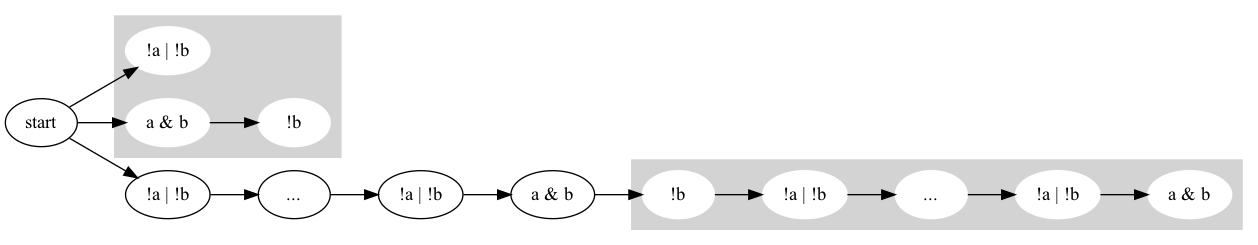
\includegraphics[scale=0.3]{examples/ex14/ex14.png}

            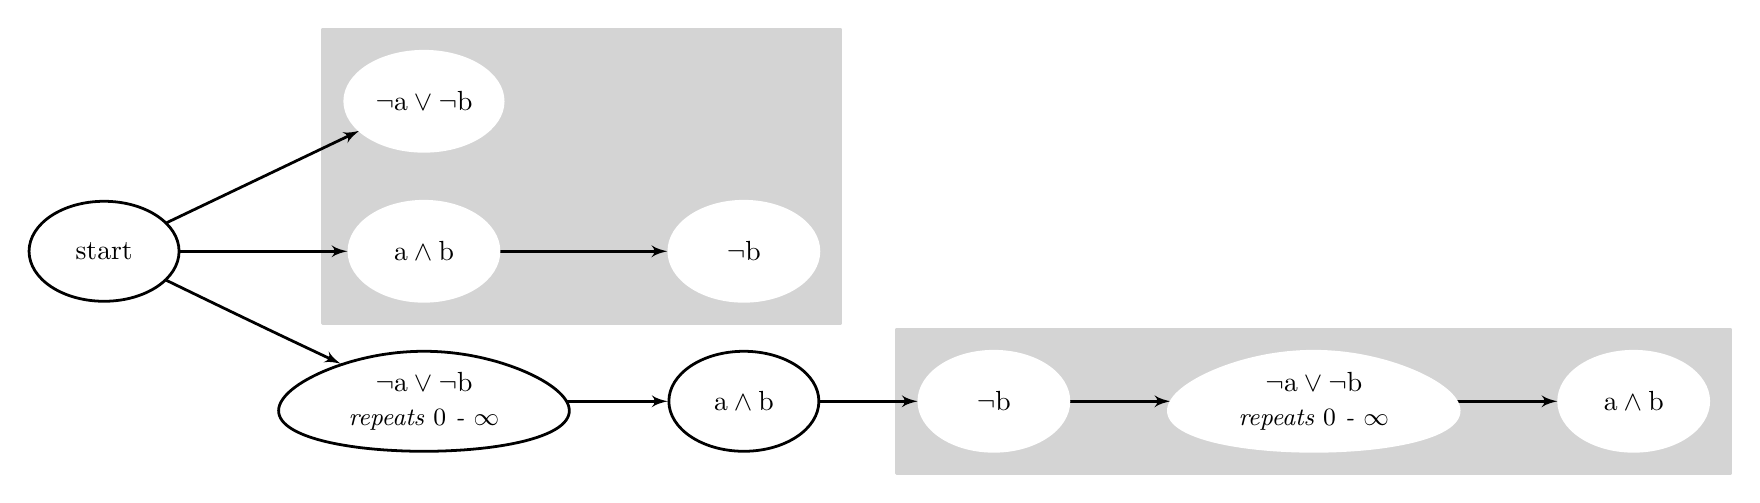
\begin{tikzpicture}[>=latex',line join=bevel,]
                \pgfsetlinewidth{1bp}
              %%
              \begin{scope}
                \pgfsetstrokecolor{black}
                \definecolor{strokecol}{rgb}{0.83,0.83,0.83};
                \pgfsetstrokecolor{strokecol}
                \definecolor{fillcol}{rgb}{0.83,0.83,0.83};
                \pgfsetfillcolor{fillcol}
                \filldraw (105.66bp,62.0bp) -- (105.66bp,168.0bp) -- (292.33bp,168.0bp) -- (292.33bp,62.0bp) -- cycle;
              \end{scope}
              \begin{scope}
                \pgfsetstrokecolor{black}
                \definecolor{strokecol}{rgb}{0.83,0.83,0.83};
                \pgfsetstrokecolor{strokecol}
                \definecolor{fillcol}{rgb}{0.83,0.83,0.83};
                \pgfsetfillcolor{fillcol}
                \filldraw (312.33bp,8.0bp) -- (312.33bp,60.0bp) -- (612.66bp,60.0bp) -- (612.66bp,8.0bp) -- cycle;
              \end{scope}
                \pgfsetcolor{black}
                % Edge: 1 -> 2
                \draw [->] (169.41bp,88.0bp) .. controls (184.02bp,88.0bp) and (202.45bp,88.0bp)  .. (229.83bp,88.0bp);
                % Edge: 5 -> 6
                \draw [->] (374.57bp,34.0bp) .. controls (382.11bp,34.0bp) and (390.67bp,34.0bp)  .. (410.91bp,34.0bp);
                % Edge: 6 -> 7
                \draw [->] (514.12bp,34.0bp) .. controls (522.4bp,34.0bp) and (530.86bp,34.0bp)  .. (550.25bp,34.0bp);
                % Edge: start -> 0
                \draw [->] (49.552bp,98.284bp) .. controls (66.247bp,106.25bp) and (89.652bp,117.42bp)  .. (118.92bp,131.39bp);
                % Edge: start -> 1
                \draw [->] (54.247bp,88.0bp) .. controls (68.853bp,88.0bp) and (87.288bp,88.0bp)  .. (114.67bp,88.0bp);
                % Edge: start -> 3
                \draw [->] (49.489bp,77.523bp) .. controls (61.408bp,71.732bp) and (76.506bp,64.429bp)  .. (90.0bp,58.0bp) .. controls (93.924bp,56.131bp) and (98.021bp,54.19bp)  .. (112.18bp,47.52bp);
                % Edge: 3 -> 4
                \draw [->] (193.79bp,34.0bp) .. controls (202.07bp,34.0bp) and (210.53bp,34.0bp)  .. (229.93bp,34.0bp);
                % Edge: 4 -> 5
                \draw [->] (284.73bp,34.0bp) .. controls (292.21bp,34.0bp) and (300.51bp,34.0bp)  .. (319.94bp,34.0bp);
                % Node: 0
              \begin{scope}
                \definecolor{strokecol}{rgb}{1.0,1.0,1.0};
                \pgfsetstrokecolor{strokecol}
                \definecolor{fillcol}{rgb}{1.0,1.0,1.0};
                \pgfsetfillcolor{fillcol}
                \filldraw [opacity=1] (142.16bp,142.0bp) ellipse (28.5bp and 18.0bp);
                \definecolor{strokecol}{rgb}{0.0,0.0,0.0};
                \pgfsetstrokecolor{strokecol}
                \draw (142.16bp,142.0bp) node {$\neg \text{a} \lor \neg \text{b}$};
              \end{scope}
                % Node: 1
              \begin{scope}
                \definecolor{strokecol}{rgb}{1.0,1.0,1.0};
                \pgfsetstrokecolor{strokecol}
                \definecolor{fillcol}{rgb}{1.0,1.0,1.0};
                \pgfsetfillcolor{fillcol}
                \filldraw [opacity=1] (142.16bp,88.0bp) ellipse (27.0bp and 18.0bp);
                \definecolor{strokecol}{rgb}{0.0,0.0,0.0};
                \pgfsetstrokecolor{strokecol}
                \draw (142.16bp,88.0bp) node {$\text{a} \land \text{b}$};
              \end{scope}
                % Node: 2
              \begin{scope}
                \definecolor{strokecol}{rgb}{1.0,1.0,1.0};
                \pgfsetstrokecolor{strokecol}
                \definecolor{fillcol}{rgb}{1.0,1.0,1.0};
                \pgfsetfillcolor{fillcol}
                \filldraw [opacity=1] (257.33bp,88.0bp) ellipse (27.0bp and 18.0bp);
                \definecolor{strokecol}{rgb}{0.0,0.0,0.0};
                \pgfsetstrokecolor{strokecol}
                \draw (257.33bp,88.0bp) node {$\neg \text{b}$};
              \end{scope}
                % Node: 5
              \begin{scope}
                \definecolor{strokecol}{rgb}{1.0,1.0,1.0};
                \pgfsetstrokecolor{strokecol}
                \definecolor{fillcol}{rgb}{1.0,1.0,1.0};
                \pgfsetfillcolor{fillcol}
                \filldraw [opacity=1] (347.33bp,34.0bp) ellipse (27.0bp and 18.0bp);
                \definecolor{strokecol}{rgb}{0.0,0.0,0.0};
                \pgfsetstrokecolor{strokecol}
                \draw (347.33bp,34.0bp) node {$\neg \text{b}$};
              \end{scope}
                % Node: 6
              \begin{scope}
                \definecolor{strokecol}{rgb}{1.0,1.0,1.0};
                \pgfsetstrokecolor{strokecol}
                \definecolor{fillcol}{rgb}{1.0,1.0,1.0};
                \pgfsetfillcolor{fillcol}
                \filldraw (467.33bp,16.05bp) -- (470.54bp,16.15bp) -- (473.71bp,16.3bp) -- (476.84bp,16.49bp) -- (479.91bp,16.74bp) -- (482.9bp,17.03bp) -- (485.82bp,17.36bp) -- (488.64bp,17.75bp) -- (491.35bp,18.18bp) -- (493.95bp,18.65bp) -- (496.43bp,19.16bp) -- (498.77bp,19.71bp) -- (500.97bp,20.31bp) -- (503.03bp,20.94bp) -- (504.93bp,21.61bp) -- (506.67bp,22.31bp) -- (508.24bp,23.04bp) -- (509.65bp,23.8bp) -- (510.9bp,24.59bp) -- (511.97bp,25.41bp) -- (512.86bp,26.25bp) -- (513.59bp,27.11bp) -- (514.15bp,27.99bp) -- (514.54bp,28.89bp) -- (514.76bp,29.8bp) -- (514.82bp,30.72bp) -- (514.72bp,31.65bp) -- (514.47bp,32.59bp) -- (514.07bp,33.53bp) -- (513.52bp,34.47bp) -- (512.84bp,35.41bp) -- (512.02bp,36.35bp) -- (511.08bp,37.28bp) -- (510.03bp,38.2bp) -- (508.86bp,39.11bp) -- (507.59bp,40.01bp) -- (506.22bp,40.89bp) -- (504.76bp,41.75bp) -- (503.22bp,42.59bp) -- (501.6bp,43.41bp) -- (499.92bp,44.2bp) -- (498.17bp,44.96bp) -- (496.36bp,45.69bp) -- (494.51bp,46.39bp) -- (492.61bp,47.06bp) -- (490.67bp,47.69bp) -- (488.7bp,48.29bp) -- (486.69bp,48.84bp) -- (484.66bp,49.35bp) -- (482.61bp,49.82bp) -- (480.53bp,50.25bp) -- (478.44bp,50.64bp) -- (476.34bp,50.97bp) -- (474.23bp,51.26bp) -- (472.1bp,51.51bp) -- (469.98bp,51.7bp) -- (467.84bp,51.85bp) -- (465.7bp,51.95bp) -- (463.56bp,52.0bp) -- (461.42bp,52.0bp) -- (459.28bp,51.95bp) -- (457.14bp,51.85bp) -- (455.01bp,51.7bp) -- (452.88bp,51.51bp) -- (450.76bp,51.26bp) -- (448.64bp,50.97bp) -- (446.54bp,50.64bp) -- (444.45bp,50.25bp) -- (442.38bp,49.82bp) -- (440.33bp,49.35bp) -- (438.29bp,48.84bp) -- (436.29bp,48.29bp) -- (434.31bp,47.69bp) -- (432.37bp,47.06bp) -- (430.47bp,46.39bp) -- (428.62bp,45.69bp) -- (426.82bp,44.96bp) -- (425.07bp,44.2bp) -- (423.38bp,43.41bp) -- (421.77bp,42.59bp) -- (420.23bp,41.75bp) -- (418.77bp,40.89bp) -- (417.4bp,40.01bp) -- (416.13bp,39.11bp) -- (414.96bp,38.2bp) -- (413.9bp,37.28bp) -- (412.96bp,36.35bp) -- (412.15bp,35.41bp) -- (411.46bp,34.47bp) -- (410.92bp,33.53bp) -- (410.52bp,32.59bp) -- (410.26bp,31.65bp) -- (410.16bp,30.72bp) -- (410.22bp,29.8bp) -- (410.45bp,28.89bp) -- (410.83bp,27.99bp) -- (411.39bp,27.11bp) -- (412.12bp,26.25bp) -- (413.02bp,25.41bp) -- (414.09bp,24.59bp) -- (415.33bp,23.8bp) -- (416.74bp,23.04bp) -- (418.32bp,22.31bp) -- (420.06bp,21.61bp) -- (421.96bp,20.94bp) -- (424.01bp,20.31bp) -- (426.21bp,19.71bp) -- (428.56bp,19.16bp) -- (431.03bp,18.65bp) -- (433.63bp,18.18bp) -- (436.35bp,17.75bp) -- (439.17bp,17.36bp) -- (442.08bp,17.03bp) -- (445.08bp,16.74bp) -- (448.14bp,16.49bp) -- (451.27bp,16.3bp) -- (454.44bp,16.15bp) -- (457.65bp,16.05bp) -- (460.88bp,16.0bp) -- (464.11bp,16.0bp) -- cycle;
                \definecolor{strokecol}{rgb}{0.0,0.0,0.0};
                \pgfsetstrokecolor{strokecol}
                \draw (462.49bp,34.0bp) node [align=center] {$\neg \text{a} \lor \neg \text{b}$ \\ {\small \emph{repeats $0$ - $\infty$}}};
              \end{scope}
                % Node: 7
              \begin{scope}
                \definecolor{strokecol}{rgb}{1.0,1.0,1.0};
                \pgfsetstrokecolor{strokecol}
                \definecolor{fillcol}{rgb}{1.0,1.0,1.0};
                \pgfsetfillcolor{fillcol}
                \filldraw [opacity=1] (577.66bp,34.0bp) ellipse (27.0bp and 18.0bp);
                \definecolor{strokecol}{rgb}{0.0,0.0,0.0};
                \pgfsetstrokecolor{strokecol}
                \draw (577.66bp,34.0bp) node {$\text{a} \land \text{b}$};
              \end{scope}
                % Node: start
              \begin{scope}
                \definecolor{strokecol}{rgb}{0.0,0.0,0.0};
                \pgfsetstrokecolor{strokecol}
                \draw (27.0bp,88.0bp) ellipse (27.0bp and 18.0bp);
                \draw (27.0bp,88.0bp) node {start};
              \end{scope}
                % Node: 3
              \begin{scope}
                \definecolor{strokecol}{rgb}{0.0,0.0,0.0};
                \pgfsetstrokecolor{strokecol}
                \draw (147.01bp,16.05bp) -- (150.21bp,16.15bp) -- (153.39bp,16.3bp) -- (156.51bp,16.49bp) -- (159.58bp,16.74bp) -- (162.58bp,17.03bp) -- (165.49bp,17.36bp) -- (168.31bp,17.75bp) -- (171.03bp,18.18bp) -- (173.63bp,18.65bp) -- (176.1bp,19.16bp) -- (178.44bp,19.71bp) -- (180.64bp,20.31bp) -- (182.7bp,20.94bp) -- (184.6bp,21.61bp) -- (186.34bp,22.31bp) -- (187.92bp,23.04bp) -- (189.33bp,23.8bp) -- (190.57bp,24.59bp) -- (191.64bp,25.41bp) -- (192.54bp,26.25bp) -- (193.26bp,27.11bp) -- (193.82bp,27.99bp) -- (194.21bp,28.89bp) -- (194.43bp,29.8bp) -- (194.49bp,30.72bp) -- (194.39bp,31.65bp) -- (194.14bp,32.59bp) -- (193.74bp,33.53bp) -- (193.19bp,34.47bp) -- (192.51bp,35.41bp) -- (191.69bp,36.35bp) -- (190.75bp,37.28bp) -- (189.7bp,38.2bp) -- (188.53bp,39.11bp) -- (187.26bp,40.01bp) -- (185.89bp,40.89bp) -- (184.43bp,41.75bp) -- (182.89bp,42.59bp) -- (181.27bp,43.41bp) -- (179.59bp,44.2bp) -- (177.84bp,44.96bp) -- (176.04bp,45.69bp) -- (174.18bp,46.39bp) -- (172.28bp,47.06bp) -- (170.34bp,47.69bp) -- (168.37bp,48.29bp) -- (166.36bp,48.84bp) -- (164.33bp,49.35bp) -- (162.28bp,49.82bp) -- (160.2bp,50.25bp) -- (158.12bp,50.64bp) -- (156.01bp,50.97bp) -- (153.9bp,51.26bp) -- (151.78bp,51.51bp) -- (149.65bp,51.7bp) -- (147.51bp,51.85bp) -- (145.37bp,51.95bp) -- (143.23bp,52.0bp) -- (141.09bp,52.0bp) -- (138.95bp,51.95bp) -- (136.82bp,51.85bp) -- (134.68bp,51.7bp) -- (132.55bp,51.51bp) -- (130.43bp,51.26bp) -- (128.32bp,50.97bp) -- (126.21bp,50.64bp) -- (124.12bp,50.25bp) -- (122.05bp,49.82bp) -- (120.0bp,49.35bp) -- (117.97bp,48.84bp) -- (115.96bp,48.29bp) -- (113.99bp,47.69bp) -- (112.05bp,47.06bp) -- (110.15bp,46.39bp) -- (108.29bp,45.69bp) -- (106.49bp,44.96bp) -- (104.74bp,44.2bp) -- (103.05bp,43.41bp) -- (101.44bp,42.59bp) -- (99.9bp,41.75bp) -- (98.44bp,40.89bp) -- (97.07bp,40.01bp) -- (95.8bp,39.11bp) -- (94.63bp,38.2bp) -- (93.57bp,37.28bp) -- (92.63bp,36.35bp) -- (91.82bp,35.41bp) -- (91.14bp,34.47bp) -- (90.59bp,33.53bp) -- (90.19bp,32.59bp) -- (89.93bp,31.65bp) -- (89.84bp,30.72bp) -- (89.9bp,29.8bp) -- (90.12bp,28.89bp) -- (90.51bp,27.99bp) -- (91.06bp,27.11bp) -- (91.79bp,26.25bp) -- (92.69bp,25.41bp) -- (93.76bp,24.59bp) -- (95.0bp,23.8bp) -- (96.41bp,23.04bp) -- (97.99bp,22.31bp) -- (99.73bp,21.61bp) -- (101.63bp,20.94bp) -- (103.68bp,20.31bp) -- (105.89bp,19.71bp) -- (108.23bp,19.16bp) -- (110.7bp,18.65bp) -- (113.3bp,18.18bp) -- (116.02bp,17.75bp) -- (118.84bp,17.36bp) -- (121.75bp,17.03bp) -- (124.75bp,16.74bp) -- (127.82bp,16.49bp) -- (130.94bp,16.3bp) -- (134.12bp,16.15bp) -- (137.32bp,16.05bp) -- (140.55bp,16.0bp) -- (143.78bp,16.0bp) -- cycle;
                \draw (142.16bp,34.0bp) node [align=center] {$\neg \text{a} \lor \neg \text{b}$ \\ {\small \emph{repeats $0$ - $\infty$}}};
              \end{scope}
                % Node: 4
              \begin{scope}
                \definecolor{strokecol}{rgb}{0.0,0.0,0.0};
                \pgfsetstrokecolor{strokecol}
                \draw (257.33bp,34.0bp) ellipse (27.0bp and 18.0bp);
                \draw (257.33bp,34.0bp) node {$\text{a} \land \text{b}$};
              \end{scope}
              %
              \end{tikzpicture}}

     %   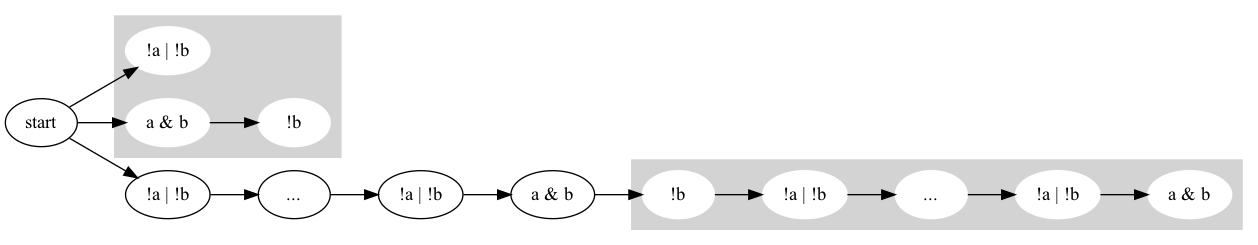
\includegraphics[scale=0.3]{examples/ex14/ex14.png}
        \caption{Timeline for $\always (a \land b \limplies \nextt (\neg b))$.}
        \label{fig:ex14}
    \end{figure*}
\end{example}

\begin{example}
    SPOT~\cite{SPOT-online} includes a command-line tool for random LTL formula generation called \texttt{randltl}~\cite{duret.13.atva}. We used it to generate the following LTL formula.
    \[
    p_2 \land (\eventually \always p_0 \stronguntil \nextt(\always p_1 \land (((p_0 \limplies p_2) \land (p_2 \limplies p_0)) \stronguntil \eventually p_0)))
    \]
    This formula is reasonably complicated, and hard for humans to reason about directly. For this LTL formula, our tool generates the timeline representation in \cref{fig:ex13}.
    \begin{figure*}[h!]
        \centering
        \resizebox{\textwidth}{!}{
            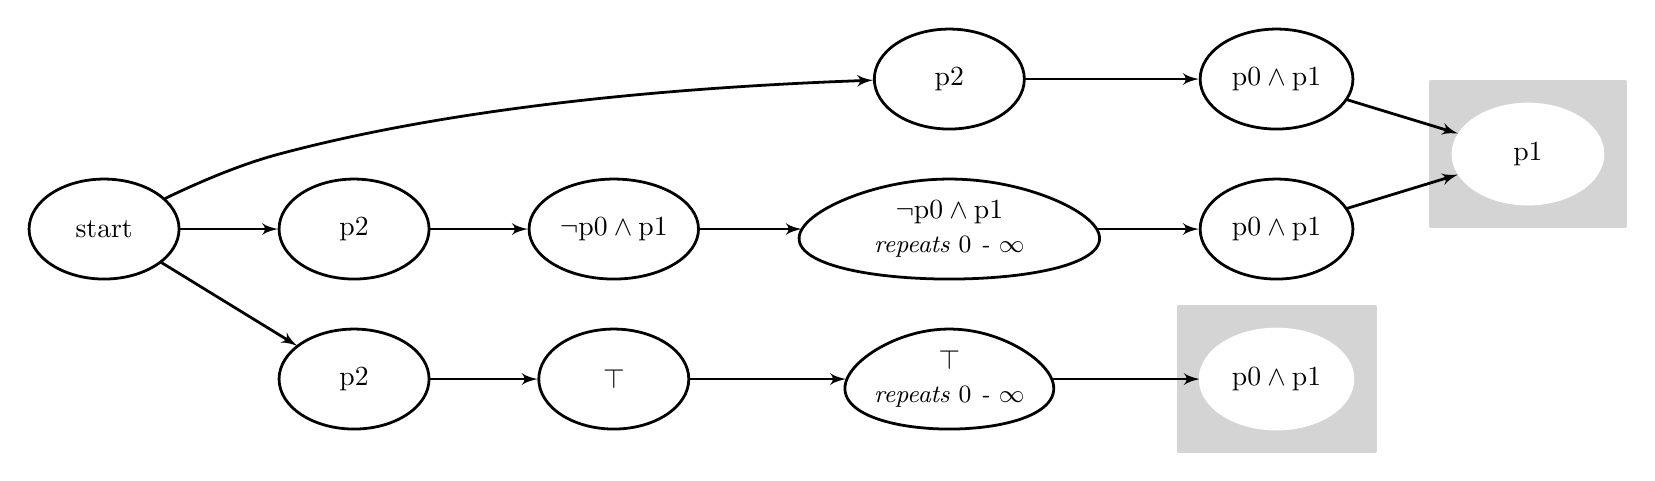
\begin{tikzpicture}[>=latex',line join=bevel,]
                \pgfsetlinewidth{1bp}
              %%
              \begin{scope}
                \pgfsetstrokecolor{black}
                \definecolor{strokecol}{rgb}{0.83,0.83,0.83};
                \pgfsetstrokecolor{strokecol}
                \definecolor{fillcol}{rgb}{0.83,0.83,0.83};
                \pgfsetfillcolor{fillcol}
                \filldraw (504.59bp,89.0bp) -- (504.59bp,141.0bp) -- (574.59bp,141.0bp) -- (574.59bp,89.0bp) -- cycle;
              \end{scope}
              \begin{scope}
                \pgfsetstrokecolor{black}
                \definecolor{strokecol}{rgb}{0.83,0.83,0.83};
                \pgfsetstrokecolor{strokecol}
                \definecolor{fillcol}{rgb}{0.83,0.83,0.83};
                \pgfsetfillcolor{fillcol}
                \filldraw (413.59bp,8.0bp) -- (413.59bp,60.0bp) -- (484.59bp,60.0bp) -- (484.59bp,8.0bp) -- cycle;
              \end{scope}
                \pgfsetcolor{black}
                % Edge: start -> 0
                \draw [->] (48.953bp,98.996bp) .. controls (60.709bp,104.68bp) and (75.823bp,111.21bp)  .. (90.0bp,115.0bp) .. controls (159.91bp,133.7bp) and (244.63bp,139.46bp)  .. (303.86bp,141.59bp);
                % Edge: start -> 2
                \draw [->] (54.403bp,88.0bp) .. controls (61.886bp,88.0bp) and (70.183bp,88.0bp)  .. (89.616bp,88.0bp);
                % Edge: start -> 7
                \draw [->] (47.53bp,76.016bp) .. controls (59.151bp,68.885bp) and (74.111bp,59.705bp)  .. (96.525bp,45.951bp);
                % Edge: 0 -> 1
                \draw [->] (358.57bp,142.0bp) .. controls (373.75bp,142.0bp) and (393.11bp,142.0bp)  .. (421.11bp,142.0bp);
                % Edge: 1 -> 6
                \draw [->] (474.27bp,134.62bp) .. controls (483.34bp,131.85bp) and (493.84bp,128.65bp)  .. (514.43bp,122.37bp);
                % Edge: 2 -> 3
                \draw [->] (144.47bp,88.0bp) .. controls (151.84bp,88.0bp) and (160.04bp,88.0bp)  .. (179.56bp,88.0bp);
                % Edge: 3 -> 4
                \draw [->] (241.48bp,88.0bp) .. controls (249.31bp,88.0bp) and (258.05bp,88.0bp)  .. (278.13bp,88.0bp);
                % Edge: 4 -> 5
                \draw [->] (384.77bp,88.0bp) .. controls (393.21bp,88.0bp) and (401.81bp,88.0bp)  .. (421.1bp,88.0bp);
                % Edge: 5 -> 6
                \draw [->] (474.27bp,95.378bp) .. controls (483.34bp,98.146bp) and (493.84bp,101.35bp)  .. (514.43bp,107.63bp);
                % Edge: 7 -> 8
                \draw [->] (144.47bp,34.0bp) .. controls (153.0bp,34.0bp) and (162.63bp,34.0bp)  .. (183.09bp,34.0bp);
                % Edge: 8 -> 9
                \draw [->] (237.86bp,34.0bp) .. controls (251.05bp,34.0bp) and (267.41bp,34.0bp)  .. (294.09bp,34.0bp);
                % Edge: 9 -> 10
                \draw [->] (368.61bp,34.0bp) .. controls (381.85bp,34.0bp) and (396.84bp,34.0bp)  .. (421.45bp,34.0bp);
                % Node: 6
              \begin{scope}
                \definecolor{strokecol}{rgb}{1.0,1.0,1.0};
                \pgfsetstrokecolor{strokecol}
                \definecolor{fillcol}{rgb}{1.0,1.0,1.0};
                \pgfsetfillcolor{fillcol}
                \filldraw [opacity=1] (539.59bp,115.0bp) ellipse (27.0bp and 18.0bp);
                \definecolor{strokecol}{rgb}{0.0,0.0,0.0};
                \pgfsetstrokecolor{strokecol}
                \draw (539.59bp,115.0bp) node {$\text{p1}$};
              \end{scope}
                % Node: 10
              \begin{scope}
                \definecolor{strokecol}{rgb}{1.0,1.0,1.0};
                \pgfsetstrokecolor{strokecol}
                \definecolor{fillcol}{rgb}{1.0,1.0,1.0};
                \pgfsetfillcolor{fillcol}
                \filldraw [opacity=1] (449.09bp,34.0bp) ellipse (27.5bp and 18.0bp);
                \definecolor{strokecol}{rgb}{0.0,0.0,0.0};
                \pgfsetstrokecolor{strokecol}
                \draw (449.09bp,34.0bp) node {$\text{p0} \land \text{p1}$};
              \end{scope}
                % Node: start
              \begin{scope}
                \definecolor{strokecol}{rgb}{0.0,0.0,0.0};
                \pgfsetstrokecolor{strokecol}
                \draw (27.0bp,88.0bp) ellipse (27.0bp and 18.0bp);
                \draw (27.0bp,88.0bp) node {start};
              \end{scope}
                % Node: 0
              \begin{scope}
                \definecolor{strokecol}{rgb}{0.0,0.0,0.0};
                \pgfsetstrokecolor{strokecol}
                \draw (331.29bp,142.0bp) ellipse (27.0bp and 18.0bp);
                \draw (331.29bp,142.0bp) node {$\text{p2}$};
              \end{scope}
                % Node: 2
              \begin{scope}
                \definecolor{strokecol}{rgb}{0.0,0.0,0.0};
                \pgfsetstrokecolor{strokecol}
                \draw (117.0bp,88.0bp) ellipse (27.0bp and 18.0bp);
                \draw (117.0bp,88.0bp) node {$\text{p2}$};
              \end{scope}
                % Node: 7
              \begin{scope}
                \definecolor{strokecol}{rgb}{0.0,0.0,0.0};
                \pgfsetstrokecolor{strokecol}
                \draw (117.0bp,34.0bp) ellipse (27.0bp and 18.0bp);
                \draw (117.0bp,34.0bp) node {$\text{p2}$};
              \end{scope}
                % Node: 1
              \begin{scope}
                \definecolor{strokecol}{rgb}{0.0,0.0,0.0};
                \pgfsetstrokecolor{strokecol}
                \draw (449.09bp,142.0bp) ellipse (27.5bp and 18.0bp);
                \draw (449.09bp,142.0bp) node {$\text{p0} \land \text{p1}$};
              \end{scope}
                % Node: 3
              \begin{scope}
                \definecolor{strokecol}{rgb}{0.0,0.0,0.0};
                \pgfsetstrokecolor{strokecol}
                \draw (210.5bp,88.0bp) ellipse (30.5bp and 18.0bp);
                \draw (210.5bp,88.0bp) node {$\neg \text{p0} \land \text{p1}$};
              \end{scope}
                % Node: 4
              \begin{scope}
                \definecolor{strokecol}{rgb}{0.0,0.0,0.0};
                \pgfsetstrokecolor{strokecol}
                \draw (336.3bp,70.05bp) -- (339.61bp,70.15bp) -- (342.89bp,70.3bp) -- (346.12bp,70.49bp) -- (349.29bp,70.74bp) -- (352.39bp,71.03bp) -- (355.4bp,71.36bp) -- (358.32bp,71.75bp) -- (361.12bp,72.18bp) -- (363.81bp,72.65bp) -- (366.37bp,73.16bp) -- (368.79bp,73.71bp) -- (371.07bp,74.31bp) -- (373.19bp,74.94bp) -- (375.15bp,75.61bp) -- (376.95bp,76.31bp) -- (378.58bp,77.04bp) -- (380.04bp,77.8bp) -- (381.32bp,78.59bp) -- (382.43bp,79.41bp) -- (383.36bp,80.25bp) -- (384.11bp,81.11bp) -- (384.69bp,81.99bp) -- (385.09bp,82.89bp) -- (385.32bp,83.8bp) -- (385.38bp,84.72bp) -- (385.28bp,85.65bp) -- (385.02bp,86.59bp) -- (384.6bp,87.53bp) -- (384.04bp,88.47bp) -- (383.33bp,89.41bp) -- (382.49bp,90.35bp) -- (381.52bp,91.28bp) -- (380.42bp,92.2bp) -- (379.22bp,93.11bp) -- (377.9bp,94.01bp) -- (376.49bp,94.89bp) -- (374.98bp,95.75bp) -- (373.39bp,96.59bp) -- (371.72bp,97.41bp) -- (369.98bp,98.2bp) -- (368.17bp,98.96bp) -- (366.3bp,99.69bp) -- (364.39bp,100.39bp) -- (362.42bp,101.06bp) -- (360.42bp,101.69bp) -- (358.38bp,102.29bp) -- (356.3bp,102.84bp) -- (354.21bp,103.35bp) -- (352.08bp,103.82bp) -- (349.94bp,104.25bp) -- (347.78bp,104.64bp) -- (345.61bp,104.97bp) -- (343.42bp,105.26bp) -- (341.23bp,105.51bp) -- (339.03bp,105.7bp) -- (336.82bp,105.85bp) -- (334.61bp,105.95bp) -- (332.4bp,106.0bp) -- (330.19bp,106.0bp) -- (327.97bp,105.95bp) -- (325.76bp,105.85bp) -- (323.56bp,105.7bp) -- (321.36bp,105.51bp) -- (319.16bp,105.26bp) -- (316.98bp,104.97bp) -- (314.81bp,104.64bp) -- (312.65bp,104.25bp) -- (310.5bp,103.82bp) -- (308.38bp,103.35bp) -- (306.28bp,102.84bp) -- (304.21bp,102.29bp) -- (302.17bp,101.69bp) -- (300.16bp,101.06bp) -- (298.2bp,100.39bp) -- (296.28bp,99.69bp) -- (294.42bp,98.96bp) -- (292.61bp,98.2bp) -- (290.87bp,97.41bp) -- (289.2bp,96.59bp) -- (287.61bp,95.75bp) -- (286.1bp,94.89bp) -- (284.68bp,94.01bp) -- (283.37bp,93.11bp) -- (282.16bp,92.2bp) -- (281.07bp,91.28bp) -- (280.1bp,90.35bp) -- (279.26bp,89.41bp) -- (278.55bp,88.47bp) -- (277.99bp,87.53bp) -- (277.57bp,86.59bp) -- (277.31bp,85.65bp) -- (277.21bp,84.72bp) -- (277.27bp,83.8bp) -- (277.5bp,82.89bp) -- (277.9bp,81.99bp) -- (278.48bp,81.11bp) -- (279.23bp,80.25bp) -- (280.16bp,79.41bp) -- (281.26bp,78.59bp) -- (282.55bp,77.8bp) -- (284.0bp,77.04bp) -- (285.63bp,76.31bp) -- (287.43bp,75.61bp) -- (289.4bp,74.94bp) -- (291.52bp,74.31bp) -- (293.8bp,73.71bp) -- (296.22bp,73.16bp) -- (298.77bp,72.65bp) -- (301.46bp,72.18bp) -- (304.27bp,71.75bp) -- (307.18bp,71.36bp) -- (310.19bp,71.03bp) -- (313.29bp,70.74bp) -- (316.46bp,70.49bp) -- (319.69bp,70.3bp) -- (322.97bp,70.15bp) -- (326.29bp,70.05bp) -- (329.62bp,70.0bp) -- (332.96bp,70.0bp) -- cycle;
                \draw (331.29bp,88.0bp) node [align=center] {$\neg \text{p0} \land \text{p1}$ \\ {\small \emph{repeats $0$ - $\infty$}}};
              \end{scope}
                % Node: 5
              \begin{scope}
                \definecolor{strokecol}{rgb}{0.0,0.0,0.0};
                \pgfsetstrokecolor{strokecol}
                \draw (449.09bp,88.0bp) ellipse (27.5bp and 18.0bp);
                \draw (449.09bp,88.0bp) node {$\text{p0} \land \text{p1}$};
              \end{scope}
                % Node: 8
              \begin{scope}
                \definecolor{strokecol}{rgb}{0.0,0.0,0.0};
                \pgfsetstrokecolor{strokecol}
                \draw (210.5bp,34.0bp) ellipse (27.0bp and 18.0bp);
                \draw (210.5bp,34.0bp) node {$\top$};
              \end{scope}
                % Node: 9
              \begin{scope}
                \definecolor{strokecol}{rgb}{0.0,0.0,0.0};
                \pgfsetstrokecolor{strokecol}
                \draw (334.77bp,16.05bp) -- (337.07bp,16.15bp) -- (339.35bp,16.3bp) -- (341.6bp,16.49bp) -- (343.8bp,16.74bp) -- (345.95bp,17.03bp) -- (348.05bp,17.36bp) -- (350.07bp,17.75bp) -- (352.02bp,18.18bp) -- (353.89bp,18.65bp) -- (355.67bp,19.16bp) -- (357.35bp,19.71bp) -- (358.93bp,20.31bp) -- (360.41bp,20.94bp) -- (361.77bp,21.61bp) -- (363.02bp,22.31bp) -- (364.15bp,23.04bp) -- (365.17bp,23.8bp) -- (366.06bp,24.59bp) -- (366.83bp,25.41bp) -- (367.47bp,26.25bp) -- (368.0bp,27.11bp) -- (368.4bp,27.99bp) -- (368.68bp,28.89bp) -- (368.84bp,29.8bp) -- (368.88bp,30.72bp) -- (368.81bp,31.65bp) -- (368.63bp,32.59bp) -- (368.34bp,33.53bp) -- (367.94bp,34.47bp) -- (367.45bp,35.41bp) -- (366.87bp,36.35bp) -- (366.19bp,37.28bp) -- (365.43bp,38.2bp) -- (364.6bp,39.11bp) -- (363.68bp,40.01bp) -- (362.7bp,40.89bp) -- (361.65bp,41.75bp) -- (360.55bp,42.59bp) -- (359.38bp,43.41bp) -- (358.17bp,44.2bp) -- (356.92bp,44.96bp) -- (355.62bp,45.69bp) -- (354.29bp,46.39bp) -- (352.93bp,47.06bp) -- (351.53bp,47.69bp) -- (350.11bp,48.29bp) -- (348.67bp,48.84bp) -- (347.21bp,49.35bp) -- (345.74bp,49.82bp) -- (344.25bp,50.25bp) -- (342.75bp,50.64bp) -- (341.24bp,50.97bp) -- (339.72bp,51.26bp) -- (338.2bp,51.51bp) -- (336.67bp,51.7bp) -- (335.13bp,51.85bp) -- (333.6bp,51.95bp) -- (332.06bp,52.0bp) -- (330.52bp,52.0bp) -- (328.99bp,51.95bp) -- (327.45bp,51.85bp) -- (325.92bp,51.7bp) -- (324.39bp,51.51bp) -- (322.86bp,51.26bp) -- (321.35bp,50.97bp) -- (319.84bp,50.64bp) -- (318.34bp,50.25bp) -- (316.85bp,49.82bp) -- (315.37bp,49.35bp) -- (313.91bp,48.84bp) -- (312.47bp,48.29bp) -- (311.05bp,47.69bp) -- (309.66bp,47.06bp) -- (308.3bp,46.39bp) -- (306.96bp,45.69bp) -- (305.67bp,44.96bp) -- (304.41bp,44.2bp) -- (303.2bp,43.41bp) -- (302.04bp,42.59bp) -- (300.93bp,41.75bp) -- (299.89bp,40.89bp) -- (298.9bp,40.01bp) -- (297.99bp,39.11bp) -- (297.15bp,38.2bp) -- (296.39bp,37.28bp) -- (295.72bp,36.35bp) -- (295.13bp,35.41bp) -- (294.64bp,34.47bp) -- (294.25bp,33.53bp) -- (293.96bp,32.59bp) -- (293.78bp,31.65bp) -- (293.71bp,30.72bp) -- (293.75bp,29.8bp) -- (293.91bp,28.89bp) -- (294.19bp,27.99bp) -- (294.59bp,27.11bp) -- (295.11bp,26.25bp) -- (295.76bp,25.41bp) -- (296.53bp,24.59bp) -- (297.42bp,23.8bp) -- (298.43bp,23.04bp) -- (299.56bp,22.31bp) -- (300.81bp,21.61bp) -- (302.18bp,20.94bp) -- (303.65bp,20.31bp) -- (305.24bp,19.71bp) -- (306.92bp,19.16bp) -- (308.7bp,18.65bp) -- (310.56bp,18.18bp) -- (312.51bp,17.75bp) -- (314.54bp,17.36bp) -- (316.63bp,17.03bp) -- (318.78bp,16.74bp) -- (320.99bp,16.49bp) -- (323.23bp,16.3bp) -- (325.51bp,16.15bp) -- (327.82bp,16.05bp) -- (330.13bp,16.0bp) -- (332.45bp,16.0bp) -- cycle;
                \draw (331.29bp,34.0bp) node [align=center] {$\top$ \\ {\small \emph{repeats $0$ - $\infty$}}};
              \end{scope}
              %
              \end{tikzpicture}}

   %     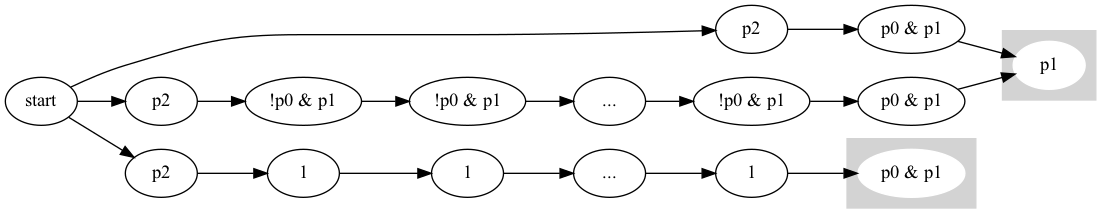
\includegraphics[scale=0.3]{examples/ex13/ex13.png}
        \caption{Timeline for $p_2 \land (\eventually \always p_0 \stronguntil \nextt(\always p_1 \land (((p_0 \limplies p_2) \land (p_2 \limplies p_0)) \stronguntil \eventually p_0)))$.}
        \label{fig:ex13}
    \end{figure*}
\end{example}
\begin{remark}
    These two examples show that our tool can generate reasonably intuitive diagrams for both real-world and randomly-generated formulas.
\end{remark}

\begin{example}
  Suppose we have the specification ``$p$ oscillates every time step.'' Human specifiers often write one of the following two LTL formulas to describe this specification.
  \begin{itemize}
    \item $\always ((p \land \nextt (\lnot p)) \lor ((\lnot p) \land \nextt p))$
    \item $\always ((p \land \nextt (\lnot p)) \land ((\lnot p) \land \nextt p))$
  \end{itemize}
  It may be hard, without rigorous analysis, to distinguish which one faithfully represents the specification. However, \tool\ generates the two timelines for these two formulas shown in \cref{fig:oscillates1,fig:oscillates2}, which clearly show the first formula is correct and the second formula is equivalent to $\bot$.
\begin{figure}[!h]
  \centering
  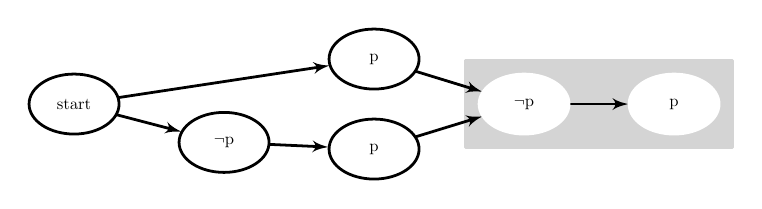
\begin{tikzpicture}[>=latex',line join=bevel,scale=0.6, transform shape]
    \pgfsetlinewidth{1bp}
  %%
  \begin{scope}
    \pgfsetstrokecolor{black}
    \definecolor{strokecol}{rgb}{0.83,0.83,0.83};
    \pgfsetstrokecolor{strokecol}
    \definecolor{fillcol}{rgb}{0.83,0.83,0.83};
    \pgfsetfillcolor{fillcol}
    \filldraw (262.0bp,19.0bp) -- (262.0bp,71.0bp) -- (422.0bp,71.0bp) -- (422.0bp,19.0bp) -- cycle;
  \end{scope}
    \pgfsetcolor{black}
    % Edge: 3 -> 4
    \draw [->] (324.4bp,45.0bp) .. controls (332.06bp,45.0bp) and (340.57bp,45.0bp)  .. (359.62bp,45.0bp);
    % Edge: start -> 0
    \draw [->] (53.503bp,48.868bp) .. controls (83.95bp,53.487bp) and (135.08bp,61.243bp)  .. (180.26bp,68.095bp);
    % Edge: start -> 1
    \draw [->] (52.513bp,38.593bp) .. controls (61.307bp,36.295bp) and (71.403bp,33.656bp)  .. (91.313bp,28.452bp);
    % Edge: 0 -> 3
    \draw [->] (232.05bp,64.622bp) .. controls (241.17bp,61.824bp) and (251.73bp,58.582bp)  .. (271.98bp,52.369bp);
    % Edge: 1 -> 2
    \draw [->] (144.4bp,20.8bp) .. controls (152.06bp,20.452bp) and (160.57bp,20.065bp)  .. (179.62bp,19.199bp);
    % Edge: 2 -> 3
    \draw [->] (232.05bp,25.378bp) .. controls (241.17bp,28.176bp) and (251.73bp,31.418bp)  .. (271.98bp,37.631bp);
    % Node: 3
  \begin{scope}
    \definecolor{strokecol}{rgb}{1.0,1.0,1.0};
    \pgfsetstrokecolor{strokecol}
    \definecolor{fillcol}{rgb}{1.0,1.0,1.0};
    \pgfsetfillcolor{fillcol}
    \filldraw [opacity=1] (297.0bp,45.0bp) ellipse (27.0bp and 18.0bp);
    \definecolor{strokecol}{rgb}{0.0,0.0,0.0};
    \pgfsetstrokecolor{strokecol}
    \draw (297.0bp,45.0bp) node {$\neg \text{p}$};
  \end{scope}
    % Node: 4
  \begin{scope}
    \definecolor{strokecol}{rgb}{1.0,1.0,1.0};
    \pgfsetstrokecolor{strokecol}
    \definecolor{fillcol}{rgb}{1.0,1.0,1.0};
    \pgfsetfillcolor{fillcol}
    \filldraw [opacity=1] (387.0bp,45.0bp) ellipse (27.0bp and 18.0bp);
    \definecolor{strokecol}{rgb}{0.0,0.0,0.0};
    \pgfsetstrokecolor{strokecol}
    \draw (387.0bp,45.0bp) node {$\text{p}$};
  \end{scope}
    % Node: start
  \begin{scope}
    \definecolor{strokecol}{rgb}{0.0,0.0,0.0};
    \pgfsetstrokecolor{strokecol}
    \draw (27.0bp,45.0bp) ellipse (27.0bp and 18.0bp);
    \draw (27.0bp,45.0bp) node {start};
  \end{scope}
    % Node: 0
  \begin{scope}
    \definecolor{strokecol}{rgb}{0.0,0.0,0.0};
    \pgfsetstrokecolor{strokecol}
    \draw (207.0bp,72.0bp) ellipse (27.0bp and 18.0bp);
    \draw (207.0bp,72.0bp) node {$\text{p}$};
  \end{scope}
    % Node: 1
  \begin{scope}
    \definecolor{strokecol}{rgb}{0.0,0.0,0.0};
    \pgfsetstrokecolor{strokecol}
    \draw (117.0bp,22.0bp) ellipse (27.0bp and 18.0bp);
    \draw (117.0bp,22.0bp) node {$\neg \text{p}$};
  \end{scope}
    % Node: 2
  \begin{scope}
    \definecolor{strokecol}{rgb}{0.0,0.0,0.0};
    \pgfsetstrokecolor{strokecol}
    \draw (207.0bp,18.0bp) ellipse (27.0bp and 18.0bp);
    \draw (207.0bp,18.0bp) node {$\text{p}$};
  \end{scope}
  %
  \end{tikzpicture}
%     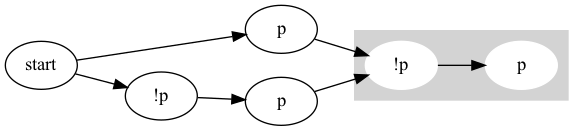
\includegraphics[scale=0.4]{examples/ex2/ex2.png}
  \caption{Timeline for $\always ((p \land \nextt (\lnot p)) \lor ((\lnot p) \land \nextt p))$.}
  \label{fig:oscillates1}
\end{figure}
\begin{figure}[!h]
  \centering
  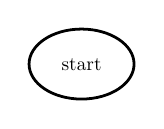
\begin{tikzpicture}[>=latex',line join=bevel, scale=0.7, transform shape]
    \pgfsetlinewidth{1bp}
  %%
  \pgfsetcolor{black}
    % Node: start
  \begin{scope}
    \definecolor{strokecol}{rgb}{0.0,0.0,0.0};
    \pgfsetstrokecolor{strokecol}
    \draw (27.0bp,18.0bp) ellipse (27.0bp and 18.0bp);
    \draw (27.0bp,18.0bp) node {start};
  \end{scope}
  %
  \end{tikzpicture}
  \caption{Timeline for $\always ((p \land \nextt (\lnot p)) \land ((\lnot p) \land \nextt p))$ (a single ``start'' means every time step is $\bot$).}
  \label{fig:oscillates2}
\end{figure}
\end{example}

\section{Playing it out} \label{sec:playing}%KYR: may swap order with the next section on artifact availability?

We quantify the usability and performance of \tool\ by compiling an extensive set of LTL formulas used in the analysis of real-life systems, defining timeline metrics, and characterizing the result of visualizing the set of real-life LTL formulas over those metrics.
% We release the set of real-life LTL formulas as a benchmark set for the research community.
Our experimental evaluation conclusively demonstrates that \tool\ scales to provide helpful visualizations of LTL formulas written by humans.


\subsection{Timeline Metrics}
\label{sec:metrics}

%KYR: Define size, length, height, complexity, etc. here.

We use two measures of complexity for timeline visualizations: timeline length and star height.
We use timeline length as a proxy for size of our timeline visualization graphs. Since Kleene stars are the trickiest operator to depict in timelines, we also use star height, a well-studied measure for the structural complexity of regular expressions, to measure the complexity of our visualizations.

\begin{definition}[Timeline Length]
    We define the timeline length of a regular expression $\tllen(A)$ recursively as follows.
    \begin{align*}
        \tllen(\emptyset)   &= -\infty\\
        \tllen(\epsilon)        &= 0\\
        \tllen(a)           &= 1\\
        \tllen(A_1 A_2)     &= \tllen(A_1) + \tllen(A_2)\\
        \tllen(A_1 + A_2)   &= \max(\tllen(A_1), \tllen(A_2))\\
        \tllen(A^*)         &= \tllen(A)
    \end{align*}
    We also extend this definition to $\omega$-regular expressions as follows.
    \begin{align*}
        \tllen(A^\omega)    &= \tllen(A)\\
        \tllen(AB)          &= \tllen(A) + \tllen(B)\\
        \tllen(B_1 + B_2)   &= \max(\tllen(B_1), \tllen(B_2))
    \end{align*}
    Then $\tllen$ captures the length of the longest path in our timeline graph visualization.
\end{definition}

\begin{definition}[Star height]
    We define the star height of regular and $\omega$-regular expressions to be the star-nesting depth in the (unsimplified) expression.
    \begin{align*}
        h(\emptyset) = h(\epsilon) = h(a) &= 0\\
        h(A_1 A_2) = h(A_1 + A_2) &= \max(h(A_1), h(A_2))\\
        h(A^*) &= 1 + h(A)\\
        h(A^\omega) &= h(A)\\
        h(A B) &= \max(h(A), h(B))\\
        h(B_1 + B_2) &= \max(h(B_1), h(B_2))
    \end{align*}

\end{definition}

\subsection{Experimental Analysis} %We could come up with a less-generic name for this, which would be nicer...

%KYR: Here we nicely show (with pictures as much as possible) all of the individual statistics and results we gathered (note aggregation occurs below).
%\paragraph{Real-world datasets}
We study the feasibility of our tool on a benchmark suite of LTL formulas gathered from real world use cases.
%
We gather a test suite totalling 91 formulas from two real-world requirement specification applications. We take $6$ specifications from NASA's Automated Airspace Concept (AAC)~\cite{GCMTR16}. We also collect formulas from the Acacia suite of examples~\cite{RV10}. We reap $85$ formulas from the suite of $23$ examples, by generating separate visualizations for each line of specification. We choose to visualize each formula individually, rather than visualize a complete set of (conjuncted) specifications, as a complete specification set may describe a large, complex system, and we only target the use case of validating individual formulas. % We choose to visualize each formula specifically, rather than complete specifications, as

We run \texttt{ltl2regex} on these $91$ examples: $87$ of the $91$ input formulas complete execution within a timeout of $20$s. Within the $87$, two examples have regular expressions of star height $8$ and are intractable to generate graph visualizations of. We are able to generate tractable visualization on the remaining $85$, or over $93\%$ of benchmarks tested. The plots of visualization complexity on these formula are provided below in \cref{fig:real-world}.


\begin{figure}[h!]
    \centering
    \subfloat{{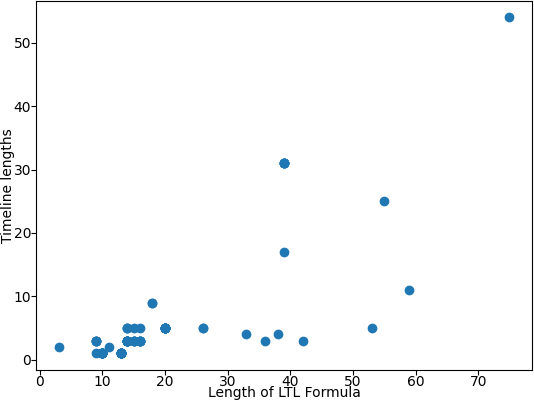
\includegraphics[width=0.49\textwidth]{img/tllens-graph.png} }}%
    \quad % [\centering label 1]
    \subfloat{{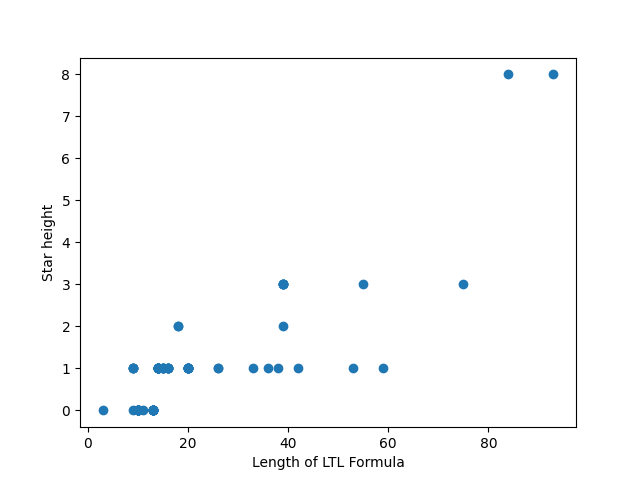
\includegraphics[width=0.49\textwidth]{img/star-height-graph.png}}}
    \caption{Visualization complexity metrics for formulas collected from Acacia~\cite{RV10} and NASA's  AAC~\cite{GCMTR16}.}
    \label{fig:real-world}
\end{figure}

%\paragraph{Scalability}
{\bf Scalability.}
%KYR: FIX!!!
We measure the scalability of our tool by running it against a set of scalable LTL formulas. We define a scalable LTL formula as one that describes an $n$-bit number using a binary counter, as generated by~\cite{RV10}. As $n$ gets larger, the LTL formula required to encode the $n$-bit counter scales in size. \cref{fig:scalability} shows that the timeline length grows approximately exponentially with the number of bits in the counter, which matches the result in Rozier and Vardi~\cite{RV10}.

In \cref{fig:scalability}, the $x$-axis ranges from $1$ to $6$, after which point it hits the $30$ seconds timeout we set, as the timeline length grows exponentially fast.

%KYR: FIX: is timeout 20 seconds or 30 seconds?!?!?

\begin{figure}[h!]
    \centering
    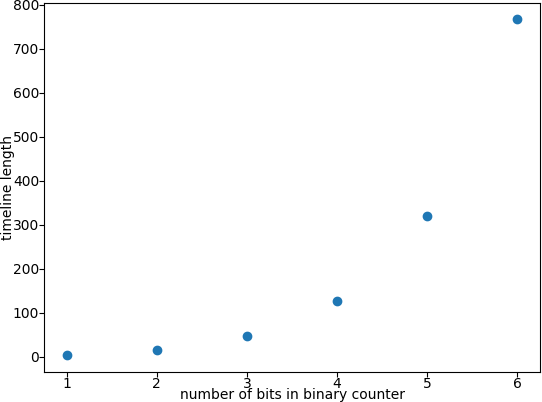
\includegraphics[width=0.49\textwidth]{img/binary.png}
    \caption{Scalability measured with binary counter examples from Rozier and Vardi~\cite{RV10}.}
    \label{fig:scalability}
\end{figure}

% KYR: Here we characterize the size of the timeline as a function of the number of bits of a binary counter for each of the four binary counter LTL formulas. The point is that these four are the only (unboundedly) scalable formulas that describe something real (i.e., they describe a binary counter for any number of bits) that have ever been published in the literature. These would throw off our metrics about the set of real LTL formulas if we included them in there. Thus, we analyze them separately, and can define the timeline size as a function of the number of bits for each of the four formulas. We can give an example or two here, such as two pictures of timelines for a 2-bit and a 3-bit counter from two different formulas, one with U's and one with X's; one with carry and one without (such as a 2-bit w/carry X formula and a 3-bit no carry U formula). The scalable counter formulas are from~\cite{RV10}.


%\paragraph{Denouement}
%KYR: aggregate and summarize all experiments here.

%<image>
%caption: For all of the <large number> of real LTL formulas historically used to analyze real systems, \tool efficiently yields usable, readable timeline visualizations.



\section{Artifact Availability: ``Thought is free\textsuperscript{\textsection}" }
\begingroup\renewcommand\thefootnote{\textsection}
\footnotetext{William Shakespeare, \emph{The Tempest}}
\endgroup
The tool we present in this paper is available at
\[
    \texttt{\url{https://github.com/EULIR/ltl-explainability}}
\]
which comes with two command-line tools, \texttt{ltl2regex} and \tool. The specific usage of the tool can be found  \href{https://github.com/EULIR/ltl-explainability#usage}{here}.

The set of LTL formulas we used to evaluate our tool in \cref{sec:playing} can be found \href{https://github.com/EULIR/ltl-explainability/tree/main/ltl-formulas}{here}.

\section{Denouement}
Based on our results, we propose the following questions for discussions and future work:
\begin{itemize}
    \item Can there be more simplification methods as described in Section~\ref{regex-simplify}? The answer is definitely positive. For example, we can add more rule-based simplifications by finding more intuitive patterns in the generated $\omega$-regular expressions. Other simplifications are also possible; for example, if the generated $\omega$-regular expression is $r_1 + r_2$ where $r_1, r_2$ are not syntactically equivalent (or equivalent up to algebraic rules) $\omega$-regular expressions, but they accept the same set of infinite-length strings, then we can simplify this down to just $r_1$. This reduces the problem to equivalence testing on $\omega$-regular expressions, which is decidable. In a similar vein, many more simplifications may apply, but the question is how \emph{useful} are they? In the end, we have to balance the efficiency, simplicity, and understandabillity of each output visualization.
    %\item Our tool is effective at translating a wide range of LTL formulas. Even with LTL formulas with complex nesting structure are represented by relatively readable timeline visualizations.
    \item Can we define timelines more formally so that one can do this process reversely (i.e., a tool that converts timeline representation to its corresponding LTL formula)? That would be very useful in practice. However, a direct reverse of the algorithm we presented in this paper may not be viable.
\end{itemize}

Going forward, it will become important to conduct a user survey to gather data from a representative audience of system engineers regarding what timeline visualizations help most with formula validation. Specifically, we list the following questions regarding the intuitive aesthetics of timelines.
\begin{itemize}
\item {\bf Can lines in timelines be curved or do they need to be straight?} If a timeline has a curved line is that still visually, intuitively a line? Does the placement of the line matter as to whether it is intuitive for the line to be straight or curved (e.g., to save space or reduce possible visual clutter)?

\item {\bf Can there be back edges in a limited fashion (i.e., to simplify formulas) in timelines?} Most of our formulas have a star-height of 1, so if we limit the back-edge representation to only surrounding a single node, that would simplify most formulas. We can then use the expanded notation for stared formulas larger than a single proposition, thus navigating the trade-off between having a small representation and limiting the visual complexity. One criticism of this approach may be that back edges cause confusion between timeline and automata representations, and that with back edges timelines stop being intuitive with respect to the linearity of time.

\item {\bf What are intuitive representations of star-formulas and do they change depending on the formula?} Common regular expression visualizers use two ways to represent stars in regular expressions. We can represent a stared formula inside a box~\cite{B22} with related caption to indicate the repetition (similar to the design decision we made in \tool); or with back edges~\cite{A20}. Does using the box cause confusion with respect to the LTL $\Box$ operator? What is the most intuitive way to remind users of the corner case where the starred formula occurs zero times?

\item {\bf When do we choose to unroll for clarity? When do we merge parallel parts of timelines?} To merge parts of lines, we have to check for logical equivalence of the parts of the timelines we want to merge. By our algorithm, we generate parallel lines only when the formulas are not syntactically equivalent, so we would be guaranteed to run the more complex check for logical equivalence. In some cases, this could provide a clarifying simplification, with the cost of a repetitive computationally-expensive check. Would it make sense to offer an ``optimizing'' compilation option to users that takes longer to create a timeline representation but checks for smaller representations via logical equivalence?
\end{itemize}


\section{Epilogue}
The Achilles heel of formal verification is specification; formal methods are only as effective at verification as their specifications are at describing the essential properties to verify. Yet, specification remains the biggest bottleneck to the use of formal methods~\cite{Roz16}. LTL is one of the most popular specification logics for industrial-scale critical systems; in the space domain alone, it is currently encapsulating specifications for the development of the NASA Lunar Gateway~\cite{DBR21,DBR23}, the Air Force Research Laboratory/Collins Aerospace Spacecraft Collision Avoidance system~\cite{HDWF21}, Space Systems Finland's Attitude and Orbit Control Systems (AOCS)~\cite{ILLTV13}, and NASA/JPL's Europa Lander Mission Concept~\cite{CDRWRWL22} just to name a few.
 %
Yet the humans that need to use formal verification tools and deeply understand their results struggle to validate that LTL formulas capture the specifications they are meant to capture. A major contributor to LTL's popularity is the propensity of humans to think of requirements in terms of timelines. This inspired the creation of LTL in the first place, as a logic that ``intuitively'' represents timelines. Our work serves to reinforce that connection, enabling visualization of most realistic LTL formulas as timelines. By releasing \tool, we contribute to better validation capabilities for LTL specifications and aid the effort to make formal verification more accessible and wide-spread.
%We hope that this will assist system designers in formulating error-free specifications and thus improve the effectiveness of verification tools for LTL.

Future extensions of this work include optimizations to the algorithm and implementation to improve performance and scalability. While we have chosen visual elements that succinctly represent timelines, it would be informative to conduct a study on different possible visualizations and which of the many ways of representing different timeline elements humans find most intuitive. It is possible that factors of context, such as the type of requirement an LTL formula describes, change its optimal timeline representation.

\section*{Acknowledgements}

This work was partially supported by the National Science Foundation (NSF) under grants CCF-2015445, CAREER-1664356, and CCRI-2016592.

\appendix
\section{Concrete Syntax of \tool} \label{sec:concrete-syntax}
Recall from~\ref{ltl-defn} that we define an LTL formula as
\begin{align*}
    \varphi = & p \mid \neg \varphi \mid \varphi \land \psi \mid \varphi \lor \psi \mid \varphi \limplies \psi \mid \always \varphi \mid \eventually \varphi \mid \nextt \varphi \\ & \mid \varphi \stronguntil \psi \mid \varphi \weakrelease \psi
\end{align*}
where $p \in \AP$ and $\varphi$ and $\psi$ are LTL formulas. In our tool \tool, we use the following concrete input syntax to represent LTL formulas in ASCII text.
\[
    \begin{array}{c r l l l@{\qquad} l}
         &      & \textit{abstract syntax}              & \textit{concrete syntax}                       & \textit{description} \\
    \varphi & =  & p                                     & \texttt{p}                                     & \text{atomic prop.} \\
         & \mid & \neg \varphi                             & \texttt{!} \varphi                                & \text{negation} \\
         & \mid & \varphi \land \psi                       & \varphi \texttt{ \& } \psi                        & \text{conjunction} \\
         & \mid & \varphi \lor \psi                        & \varphi \texttt{ | } \psi                         & \text{disjunction} \\
         & \mid & \varphi \limplies \psi                   & \varphi \texttt{ -> } \psi                        & \text{implication} \\
         & \mid & \always \varphi                          & \texttt{G} \varphi                                & \text{globally} \\
         & \mid & \eventually \varphi                      & \texttt{F} \varphi                                & \text{in the future} \\
         & \mid & \nextt \varphi                           & \texttt{X} \varphi                                & \text{next} \\
         & \mid & \varphi \stronguntil \psi                & \varphi \texttt{ U } \psi                         & \text{until} \\
         & \mid & \varphi \weakrelease \psi                & \varphi \texttt{ R } \psi                         & \text{release} \\
    \end{array}
\]
%\nocite{*}
\bibliographystyle{IEEEtran}
\bibliography{RelatedWork}


\end{document}


\subsection{Set of Real LTL Formulas}

We collect the LTL formulas from a covering set of publicly-available case studies that use LTL in the analysis of real-life safety-critical systems. As some formulas are redundant (i.e., common properties occur in many different case studies), it is not necessary to include every paper that has ever used LTL in a real setting; we instead opt for the largest and most unique formulas to cover the space of realistic use of LTL.

Given the tremendous popularity of LTL as a specification language for industrial analysis, surprisingly few real-life system analysis case studies publicly release their LTL formula specifications, largely to protect proprietary system information. We purposely avoid using the random or machine-generated formulas from published benchmarks because the purpose of \tool is helping humans understand and validate LTL formulas. Thus, we gather an extensive, representative set of formulas humans have written or needed to understand. Our LTL formula collection is as follows.

\noindent
\begin{table}[h]
\begin{tabular}{p{3.6in}|c|c}
  \hline
  Purpose & \# formulas & Source \\
  \hline
  Design space for NASA's AAC (Automated Airspace Concept) & 20,250 &~\cite{GCMTR16} \\
  \hline
  Safety specifications for Boeing's AIR6110 wheel brake system & &~\cite{BCFJKPRT15} \\
  \hline
  Requirements for model checking NASA's AAC high-level architecture & 6 &~\cite{ZR14} \\
  \hline
  Real formulas collected from all publicly-available, pre-2011 case studies & 63 &~\cite{RV11} \\
  \hline
\end{tabular}
\end{table}


